%--------------------------------------------------------------------

\documentclass[
% -- opções da classe memoir --
12pt,				% tamanho da fonte
openright,			% capítulos começam em pág ímpar (insere página vazia)
twoside,			% para impressão em verso e anverso. Oposto a oneside
a4paper,			% tamanho do papel. 
oldfontcommands,
% -- opções da classe abntex2 --
chapter=TITLE,		% títulos de capítulos convertidos em letras maiúsculas
section=TITLE,		% títulos de seções convertidos em letras maiúsculas
%subsection=TITLE,	% títulos de subseções convertidos em letras maiúsculas
%subsubsection=TITLE,% títulos de subsubseções convertidos em letras maiúsculas
% -- opções do pacote babel --
french,				% idioma adicional para hifenização
spanish,			% idioma adicional para hifenização
brazil, 
english				% o último idioma é o principal do documento
]{abntex2}

% \setlength {\marginparwidth }{2cm}
% \usepackage{todonotes}
% ---
% Pacotes básicos 
% ---
%\usepackage{lmodern}% Usa a fonte Latin Modern	
\usepackage{rotating}
\usepackage{times}
\usepackage[T1]{fontenc}		% Selecao de codigos de fonte.
\usepackage[utf8]{inputenc}		% Codificacao do documento (conversão automática dos acentos)
\usepackage{lastpage}			% Usado pela Ficha catalográfica
\usepackage{indentfirst}		% Indenta o primeiro parágrafo de cada seção.
\usepackage{color}				% Controle das cores
\usepackage{graphicx}			% Inclusão de gráficos
\usepackage{microtype} 			% para melhorias de justificação
\usepackage{float}
\usepackage{subcaption}
\usepackage{multirow}
\usepackage{bigstrut}
\usepackage{booktabs}
\usepackage{listings}
\usepackage{xcolor}
\usepackage{comment}
\usepackage{pdflscape}
\usepackage{verbatimbox}
\usepackage{makecell}
\usepackage{pbox}
\usepackage{comment}
\usepackage{bm}

\usepackage{hyperref}
\hypersetup{
    colorlinks=true,
    linkcolor=blue,
    filecolor=magenta,      
    urlcolor=cyan,
    pdftitle={Overleaf Example},
    pdfpagemode=FullScreen,
    }

\urlstyle{same}


%----------------------------------------------------------------------
% Estilo de cores para códigos
\definecolor{codegreen}{rgb}{0,0.6,0}
\definecolor{codegray}{rgb}{0.5,0.5,0.5}
\definecolor{codepurple}{rgb}{0.58,0,0.82}
\definecolor{backcolour}{rgb}{0.98,0.98,0.95}

\lstdefinestyle{mystyle}{
	backgroundcolor=\color{backcolour},   
	commentstyle=\color{codegreen},
	keywordstyle=\color{magenta},
	numberstyle=\tiny\color{codegray},
	stringstyle=\color{codepurple},
	basicstyle=\ttfamily\footnotesize,
	breakatwhitespace=false,         
	breaklines=true,                 
	captionpos=b,                    
	keepspaces=true,                 
	numbers=left,                    
	numbersep=5pt,                  
	showspaces=false,                
	showstringspaces=false,
	showtabs=false,                  
	tabsize=2
}

\lstset{style=mystyle}

%----------------------------------------------------------------------
% Pacotes usados especificamente neste documento
\usepackage{amsfonts, amsmath, amsthm, amsbsy,amssymb,bm,mathtools} % For math fonts, symbols and environments %
\usepackage{graphicx} 		% Required for including images
\usepackage{transparent}	% may be required for inkscape pdf figures (http://bit.ly/18i5Oga)
\usepackage{pdfpages}
\newsubfloat{figure}		% Allow subfloats in figure environment (http://bit.ly/1C20NAj)
\graphicspath{{pictures/}}
% \usepackage[short, nocomma]{optidef}
\usepackage[ruled,vlined,english]{algorithm2e}
\usepackage{siunitx} % units package
\let\DeclareUSUnit\DeclareSIUnit
\let\US\SI
\let\us\si
\DeclareUSUnit\inch{in}
\sisetup{detect-all}  %it may be necessary to load it after loading the font package
\usepackage{cancel}

\usepackage{tikz}
\usetikzlibrary{positioning,calc,fit}
\usetikzlibrary{arrows.meta}

%----------------------------------------------------------------------
% Comandos criados pelo usuário
\newcommand{\afazer}[1]{{\color{red}{#1}}} % Para destacar uma parte a ser trabalhada
\DeclareMathOperator*{\argmin}{\arg\!\min}
\DeclareMathOperator*{\argmax}{\arg\!\max}
\newcommand{\normp}[2]{\left\lVert#1\right\rVert_{#2}}
\allowdisplaybreaks

% Number sets
\newcommand{\R}{\mathbb{R}}
\newcommand{\Z}{\mathbb{Z}}

\newcommand{\conv}{\mathrm{conv}}

% ---
% Pacotes de citações
% ---
% \usepackage[brazilian,hyperpageref]{backref}	 % Paginas com as citações na bibl
\usepackage[alf]{abntex2cite}	% Citações padrão ABNT

% --- 
% CONFIGURAÇÕES DE PACOTES
% --- 

% ---
% Configurações do pacote backref
% % Usado sem a opção hyperpageref de backref
% \renewcommand{\backrefpagesname}{Citado na(s) página(s):~}
% % Texto padrão antes do número das páginas
% \renewcommand{\backref}{}
% % Define os textos da citação
% \renewcommand*{\backrefalt}[4]{
% 	\ifcase #1 %
% 		Nenhuma citação no texto.%
% 	\or
% 		Citado na página #2.%
% 	\else
% 		Citado #1 vezes nas páginas #2.%
% 	\fi}%
% % ---

% ---
% Informações de dados para CAPA e FOLHA DE ROSTO
% ---

\titulo{Deep-learning-based Primal Heuristics for MILP:\protect\\Supervised Solution-prediction Models}

\autor{Bruno Machado Pacheco}
\local{Florianópolis}
\data{2024}
\orientador{Prof. Eduardo Camponogara, Ph.D.}
\coorientador{Prof. Laio Oriel Seman, Ph.D.}

\instituicao{%
	Universidade Federal de Santa Catarina -- UFSC
	\par
	Centro Tecnológico
	\par
	Programa de Pós-Graduação em Engenharia de Automação e Sistemas}
\tipotrabalho{Dissertação Mestrado}
% O preambulo deve conter o tipo do trabalho, o objetivo, 
% o nome da instituição e a área de concentração 
\preambulo{Dissertação submetida ao Programa de Pós-Graduação em Engenharia de Automação e Sistemas da Universidade Federal de Santa Catarina para a obtenção do título de Mestre em Engenharia de Automação e Sistemas}
% ---


% ---
% Configurações de aparência do PDF final

% alterando o aspecto da cor azul
\definecolor{blue}{RGB}{41,5,195}

% informações do PDF
\makeatletter
\hypersetup{
	%pagebackref=true,
	pdftitle={\@title}, 
	pdfauthor={\@author},
	pdfsubject={\imprimirpreambulo},
	pdfcreator={Bruno Machado Pacheco},
	pdfkeywords={abnt}{latex}{abntex}{abntex2}{trabalho acadêmico}, 
	colorlinks=false,       		% false: boxed links; true: colored links
	linkcolor=blue,          	% color of internal links
	citecolor=blue,        		% color of links to bibliography
	filecolor=magenta,      		% color of file links
	urlcolor=blue,
	bookmarksdepth=4,
	hidelinks
}
\makeatother
% --- 

% --- 
% Espaçamentos entre linhas e parágrafos 
% --- 

% O tamanho do parágrafo é dado por:
\setlength{\parindent}{1.3cm}

% Controle do espaçamento entre um parágrafo e outro:
\setlength{\parskip}{0.2cm}  % tente também \onelineskip

% ---
% compila o indice
% ---
\makeindex
% ---

% ---
% Controla quais elementos serão compilados (útil para desenvolvimento)
% ---
\includeonly{%
beforetext/agradecimentos,
beforetext/epigrafe,
beforetext/fichacatalografica,
beforetext/folhadeaprovacao,
beforetext/resumos,
beforetext/siglas,
beforetext/simbolos,
chapters/intro,
chapters/chapter_1,
chapters/chapter_2,
chapters/chapter_3,
chapters/chapter_4,
chapters/chapter_5,
chapters/chapter_6,
chapters/conclusion,
% aftertext/apendice_a,
% aftertext/anexo_a,
% aftertext/anexo_b,
}


% ----
% Início do documento
% ----
\begin{document}
	\selectlanguage{english}
	% Retira espaço extra obsoleto entre as frases.
	\frenchspacing 
	
	% ----------------------------------------------------------
	% ELEMENTOS PRÉ-TEXTUAIS
	% ----------------------------------------------------------
	% \pretextual
	
	% ---
	% Capa
	% ---
	\imprimircapa
	% ---
	
	% ---
	% Folha de rosto
	% (o * indica que haverá a ficha bibliográfica)
	% ---
	\imprimirfolhaderosto*
	% ---
	
	% ---
	% Inserir a ficha bibliografica
	% ---
	
	% Isto é um exemplo de Ficha Catalográfica, ou ``Dados internacionais de
	% catalogação-na-publicação''. Você pode utilizar este modelo como referência. 
	% Porém, provavelmente a biblioteca da sua universidade lhe fornecerá um PDF
	% com a ficha catalográfica definitiva após a defesa do trabalho. Quando estiver
	% com o documento, salve-o como PDF no diretório do seu projeto e substitua todo
	% o conteúdo de implementação deste arquivo pelo comando abaixo:
	%
	

\ifenglish

Legal Notes:

There is no warranty for any part of the documented software. The authors have taken care in the
preparation of this thesis, but make no expressed or implied warranty of any kind and assume no
responsibility for errors or omissions. No liability is assumed for incidental or consequential
damages in connection with or arising out of the use of the information or programs contained here.

\else

Notas legais:

Não há garantia para qualquer parte do software documentado. Os autores tomaram cuidado na
preparação desta tese, mas não fazem nenhuma garantia expressa ou implícita de qualquer tipo e não
assumem qualquer responsabilidade por erros ou omissões. Não se assume qualquer responsabilidade por
danos incidentais ou consequentes em conexão ou decorrentes do uso das informações ou programas aqui
contidos.

\fi


% http://portalbu.ufsc.br/ficha
% http://portal.bu.ufsc.br/servicos/ficha-de-identificacao-da-obra/
\begin{fichacatalografica}
    \vspace*{\fill}

    \begin{center}

        \lang
        {Cataloging at source by the University Library of the Federal University of Santa Catarina.}
        {Catalogação na fonte pela Biblioteca Universitária da Universidade Federal de Santa Catarina.}

        \lang
        {File compiled at \currenttime h of the day \today.}
        {Arquivo compilado às \currenttime h do dia \today.}

        \framebox[\textwidth]
        {
            % https://tex.stackexchange.com/questions/369918/use-the-value-of-title-with-removed-linebreak
            \begin{minipage}{0.98\textwidth}
            \begingroup \let\\=\space

                \ttfamily
                \imprimirautor

                \hspace{0.5cm} \imprimirtitulo%
                \ifnotempty{\imprimirsubtitulo}{~:~\imprimirsubtitulo}%
                ~/~\imprimirautor%
                ;~\imprimirorientadorRotulo,~\imprimirorientador%
                \ifnotempty{\imprimircoorientador}{;~\imprimircoorientadorRotulo,~\imprimircoorientador}%
                ~--~\imprimirlocal,~\imprimirdata.

                % Prints how much pages there are on the document and links to the last page
                \hspace{0.5cm} \pageref{LastPage} p.
                \bigskip

                \hspace{0.5cm} \imprimirtipotrabalho~--~\imprimirinstituicao,
                \imprimircentro,~\imprimirprograma.
                \bigskip

                \hspace{0.5cm} \lang{Includes references}{Inclui referências}
                \bigskip

                % https://tex.stackexchange.com/questions/54055/using-lower-case-roman-numerals-in-enumerate-lists
                % https://tex.stackexchange.com/questions/61811/how-to-define-inparaenum-in-the-preamble
                \hspace{0.5cm}
                \begin{inparaenum}
                    \lang{\palavraschaveinglescomvirgula}{\palavraschaveportuguescomvirgula}%
                \end{inparaenum}%
                \begin{inparaenum}[I.]
                    \item \imprimirorientador~
                    \ifnotempty{\imprimircoorientador}{\item \imprimircoorientador~}
                    \item \imprimirprograma~
                    \item \imprimirtitulo~
                \end{inparaenum}%
                \bigskip

                \hspace{7.75cm} CDU 02:141:005.7

            \endgroup
            \end{minipage}
        }

    \end{center}

\end{fichacatalografica}



	
	% ---
	% Inserir errata
	% ---
	% \begin{errata}
% Elemento opcional da \citeonline[4.2.1.2]{NBR14724:2011}. Exemplo:

\vspace{\onelineskip}

FERRIGNO, C. R. A. \textbf{Tratamento de neoplasias ósseas apendiculares com
reimplantação de enxerto ósseo autólogo autoclavado associado ao plasma
rico em plaquetas}: estudo crítico na cirurgia de preservação de membro em
cães. 2011. 128 f. Tese (Livre-Docência) - Faculdade de Medicina Veterinária e
Zootecnia, Universidade de São Paulo, São Paulo, 2011.

\begin{table}[htb]
\center
\footnotesize
\begin{tabular}{|p{1.4cm}|p{1cm}|p{3cm}|p{3cm}|}
  \hline
  \textbf{Folha} & \textbf{Linha}  & \textbf{Onde se lê}  & \textbf{Leia-se}  \\
    \hline
    1 & 10 & auto-conclavo & autoconclavo\\
  \hline
\end{tabular}
\end{table}

\end{errata}

	% ---
	
	% ---
	% Inserir folha de aprovação
	% ---
	
	% Isto é um exemplo de Folha de aprovação, elemento obrigatório da NBR
	% 14724/2011 (seção 4.2.1.3). Você pode utilizar este modelo até a aprovação
	% do trabalho. Após isso, substitua todo o conteúdo deste arquivo por uma
	% imagem da página assinada pela banca com o comando abaixo:
	%
	% \includepdf{folhadeaprovacao_final.pdf}
	%
	

\addtotextpreliminarycontent{\lang{Approval Sheet}{Folha de Aprovação}}

\begin{folhadeaprovacao}

    \begin{center}
        {\imprimirautor}

        \begin{center}
            \ABNTEXchapterfont\bfseries\MakeUppercase{\imprimirtitulo}\ifnotempty{\imprimirsubtitulo}{: \imprimirsubtitulo}
        \end{center}

        \begin{minipage}{\textwidth}
            \lang
            {
                This \imprimirtipotrabalho~was considered appropriate to get the \imprimirformacao,
                \ifnotempty{\imprimirarea}{in the area of \imprimirarea,}
                and it was approved by the \imprimirprograma~of \imprimircentro~of \imprimirinstituicao.
            }
            {
                Este(a) \imprimirtipotrabalho~foi julgado adequado(a) para obtenção do Título de \imprimirformacao,
                \ifnotempty{\imprimirarea}{na área de concentração de \imprimirarea,}
                e foi aprovado em sua forma final pelo \imprimirprograma~
                do \imprimircentro~da \imprimirinstituicao.
            }
         \end{minipage}%
    \end{center}

    \begin{center}
        \imprimirlocal, \imprimirdata.
    \end{center}

    \assinatura{%
        \textbf{\imprimircoordenador} \\
        \imprimircoordenadorRotulo~\lang{of}{do} \imprimirprograma
    }

    % \newpage
    \begin{flushleft}
        \textbf{\lang{Examination Board}{Banca Examinadora}:}
    \end{flushleft}

    \assinatura{%
        \textbf{\imprimirorientador} \\ \imprimirorientadorRotulo\\
        \imprimirinstituicao~--~\imprimirinstituicaosigla
    }

    \ifnotempty{\imprimircoorientador}{%
        \assinatura{%
            \textbf{\imprimircoorientador} \\ \imprimircoorientadorRotulo \\
            \imprimirinstituicao~--~\imprimirinstituicaosigla
        }
    }

    \assinatura{%
        \textbf{Prof. Convidado 1, \lang{PhD.}{Dr.}} \\
        Instituição 1 -- Sigla 1
    }

    \assinatura{%
        \textbf{Prof. Convidado 2, \lang{PhD.}{Dr.}} \\
        Instituição 2 -- Sigla 2
    }

    \assinatura{%
        \textbf{Prof. Convidado 3, \lang{PhD.}{Dr.}} \\
        Instituição 3 -- Sigla 3
    }

    \assinatura{%
        \textbf{Prof. Convidado 4, \lang{PhD.}{Dr.}} \\
        Instituição 4 -- Sigla 4
    }

\end{folhadeaprovacao}



	% ---
	
	% ---
	% Dedicatória
	% ---
	%\begin{dedicatoria}
	%	\vspace*{\fill}
	%	\centering
	%	\noindent
	%	\textit{Dedicatoria} \vspace*{\fill}
	%\end{dedicatoria}
	% ---
	
	% ---
	% Agradecimentos
	% ---
	

\addtotextpreliminarycontent{\lang{Acknowledgement}{Agradecimentos}}

\begin{agradecimentos}

\lang
{
    Greetings.
}
{
    Os agradecimentos principais são direcionados à Gerald Weber, Miguel Frasson,
    Leslie H. Watter, Bruno Parente Lima, Flávio de Vasconcellos Corrêa, Otavio Real
    Salvador, Renato Machnievscz\footnote{Os nomes dos integrantes do primeiro
    projeto abn\TeX\ foram extraídos de
    \url{http://codigolivre.org.br/projects/abntex/}} e todos aqueles que
    contribuíram para que a produção de trabalhos acadêmicos conforme
    as normas ABNT com \LaTeX{} fosse possível.

    Agradecimentos especiais são direcionados ao Centro de Pesquisa em Arquitetura
    da Informação\footnote{\url{http://www.cpai.unb.br/}} da Universidade de
    Brasília (CPAI), ao grupo de usuários
    \emph{latex-br}\footnote{\url{http://groups.google.com/group/latex-br}} e aos
    novos voluntários do grupo
    \emph{\abnTeX{}}\footnote{\url{http://groups.google.com/group/abntex2} e
    \url{http://abntex2.googlecode.com/}}~que contribuíram e que ainda
    contribuirão para a evolução do \abnTeX{}.
}

\end{agradecimentos}


%Mesmo padrão da seção primária, porém sem indicativo numérico. Assim como: Dedicatória, Resumo, Abstract, Sumário, Listas, Referências, Apêndices e Anexos.
%
%
%Corpo do texto, fonte 10,5, justificado, recuo especial da primeira linha de 1 cm, espaçamento simples.
%

	% ---
	
	% ---
	% Epígrafe
	% ---
	

\addtotextpreliminarycontent{\lang{Epigraph}{Epigrafe}}

\begin{epigrafe}

\vspace*{\fill}\lang
{
    \begin{flushright}
        \textit{``Learn from yesterday, live for today, hope for tomorrow. The important thing is not to stop questioning.''} \\ Albert Einstein
    \end{flushright}
    \begin{flushright}
        \textit{``The true sign of intelligence is not knowledge but imagination.''} \\  Albert Einstein
    \end{flushright}
    \begin{flushright}
        \textit{``Peace cannot be kept by force; it can only be achieved by understanding.''} \\ Albert Einstein
    \end{flushright}
    \begin{flushright}
        \textit{``Whoever is careless with the truth in small matters cannot be trusted with important matters.''} \\ Albert Einstein
    \end{flushright}
    \begin{flushright}
        \textit{``Extraordinary claims require extraordinary evidence''} \\ Carl Sagan
    \end{flushright}
    \begin{flushright}
        \textit{``Catholic, which I was until I reached the age of reason.''} \\ George Carlin
    \end{flushright}
    \begin{flushright}
        \textit{``We made too many wrong mistakes.''} \\ Yogi Berra
    \end{flushright}
}
{
    \begin{flushright}
        \textit{``Assim como aquele pecado da juventude, este documento te perseguirá pelo resto da vida.''} \\ Enio Valmor Kassick
    \end{flushright}
    \begin{flushright}
        \textit{``Estupidez trará mais autoconfiança do que o conhecimento e a bravura juntas. \englishword{\showfont}''} \\ Adriano Ruseler
    \end{flushright}
}

\end{epigrafe}



% 	% ---
	
	% ---
	% RESUMOS
	% ---
	
	

\newcommand{\imprimirbrazilabstract}{%
    \cleardoublepage\phantomsection
    \addtotextpreliminarycontent{Resumo em Português}
    \begin{otherlanguage*}{brazil}
    \begin{resumo}[Resumo]

        Segundo a \textcite[3.1-3.2]{NBR6028:2003}, o resumo deve ressaltar o
        objetivo, o método, os resultados e as conclusões do documento. A ordem e a extensão
        destes itens dependem do tipo de resumo (informativo ou indicativo) e do
        tratamento que cada item recebe no documento original. O resumo deve ser
        precedido da referência do documento, com exceção do resumo inserido no
        próprio documento. (\ldots) As palavras-chave devem figurar logo abaixo do
        resumo, antecedidas da expressão Palavras-chave:, separadas entre si por
        ponto e finalizadas também por ponto.

        Além disso, na UFSC o texto do resumo deve ser digitado, em um único bloco, sem espaço de parágrafo. O resumo deve
        ser significativo, composto de uma sequência de frases concisas, afirmativas e não de uma
        enumeração de tópicos. Não deve conter citações. Deve usar o verbo na voz passiva. Abaixo do
        resumo, deve-se informar as palavras-chave (palavras ou expressões significativas retiradas do
        texto) ou, termos retirados de thesaurus da área. \englishword{\showfont}

        \imprimirpalavraschave{Palavras-chaves}{\begin{inparaitem}[]\palavraschaveportugues\end{inparaitem}}

    \end{resumo}
    \end{otherlanguage*}
}


\newcommand{\imprimirenglishabstract}{%
    % https://tex.stackexchange.com/questions/20987/changing-babel-package-inside-a-single-chapter
    % https://tex.stackexchange.com/questions/36526/multiple-language-document-babel-selectlanguage-vs-begin-endotherlanguage
    \cleardoublepage\phantomsection
    \addtotextpreliminarycontent{English's Abstract}
    \begin{otherlanguage*}{english}
    \begin{resumo}[Abstract]

        This is the English abstract.

        \imprimirpalavraschave{Keywords}{\begin{inparaitem}[]\palavraschaveingles\end{inparaitem}}

    \end{resumo}
    \end{otherlanguage*}
}


% \newcommand{\imprimirfrenchabstract}{%
%     \addtotextpreliminarycontent{Français Résumé}
%     \begin{resumo}[Résumé]
%       \begin{otherlanguage*}{french}
%           Il s'agit d'un résumé en français.

%           \imprimirpalavraschave{Mots-clés}{latex. abntex. publication de textes.}
%       \end{otherlanguage*}
%     \end{resumo}
% }


% \newcommand{\imprimirspanishabstract}{%
%     \addtotextpreliminarycontent{Español Resumen}
%     \begin{resumo}[Resumen]
%       \begin{otherlanguage*}{spanish}
%           Este es el resumen en español.

%           \imprimirpalavraschave{Palabras clave}{latex. abntex. publicación de textos.}
%       \end{otherlanguage*}
%     \end{resumo}
% }


\makeatletter
\ifenglish
    \@ifundefined{imprimirbrazilabstract}{}{\imprimirbrazilabstract}

    % https://tex.stackexchange.com/questions/331108/times-new-roman-in-latex-just-some-text
    % https://tex.stackexchange.com/questions/11707/how-to-force-output-to-a-left-or-right-page
    % https://tex.stackexchange.com/questions/132966/do-not-display-chapter-title-in-memoir-class
    \cleardoublepage\phantomsection
    \pretextualchapter{Resumo Expandido}
    \addtotextpreliminarycontent{Resumo Expandido}

    \begin{otherlanguage*}{brazil}
        \setlength{\parskip}{0.2cm}
        \setlength{\parindent}{0.0cm}
        \fontfamily{ptm}\selectfont

        \section*{Introdução}
        O resumo expandido é previsto na Resolução Normativa nº 95/CUn/2017, Art. 55, § 2, de 4 de
        abril de 2017, e exigido para teses e dissertações escritas em idiomas estrangeiros (com
        exceção dos cursos pertinentes ao estudo de idiomas estrangeiros – Programa de Pós-Graduação
        em Estudos da Tradução e Programa de Pós-Graduação em Inglês: Estudos Linguísticos e
        Literários).

        O resumo expandido é considerado um elemento pré-textual e deverá ser incluído no trabalho
        após o resumo e antes do abstract. Deverá iniciar em página impar (no anverso de uma folha)
        continuando no verso da folha. O texto deverá seguir o formato A5, com margens espelhadas:
        superior 2,0 cm, inferior 1,5 cm, interna 2,5 cm e externa 1,5. Deve ser empregada a fonte
        Time New Roman.  Todo o texto deve ser digitado em tamanho 10,5. O espaçamento entre as
        linhas deverá ser simples. A expressão “resumo expandido” deve seguir a mesma tipografia das
        demais sessões primárias do trabalho.

        O texto do resumo expandido deve ser redigido em português e conter as seguintes seções (ver
        modelo): Introdução, Objetivos, Metodologia, Resultados e Discussão e Considerações Finais.
        Deve apresentar no mínimo duas (02) e, no máximo, cinco (05) páginas contendo a mesma
        formatação em A5 do resumo e do abstract, bem como palavras-chave. \englishword{\showfont}

        \section*{Objetivos}
        Lorem ipsum dolor sit amet, consectetur adipiscing elit. Phasellus vitae dolor lacus. Ut
        accumsan vitae felis nec porttitor. Integer interdum fringilla feugiat. Nullam pulvinar sit
        amet tellus eget maximus. Donec sit amet magna eget justo semper fermentum vel eget velit.
        In iaculis imperdiet mauris, ac ornare libero placerat non. Nulla libero lectus, ullamcorper
        ac ornare eget, pulvinar ac nulla. Curabitur vestibulum non nisl eget sagittis. Proin
        gravida lacus id eros bibendum interdum. Mauris ullamcorper elementum tortor sed consequat.
        Integer tempus, est a lobortis vehicula, nisi mi fringilla augue, non semper leo metus in
        quam. Etiam in leo maximus, pulvinar mi eget, vehicula risus. Donec sed dui semper, dictum
        eros at, suscipit felis.

        Nam sagittis vel orci at tempus. Nulla non pellentesque eros.
        Quisque cursus leo massa, eu ultricies nisl lacinia a. Nulla sit amet elementum ligula.
        Proin sodales venenatis dictum. Ut et est cursus, vulputate velit et, viverra odio. Interdum
        et malesuada fames ac ante ipsum primis in faucibus. Maecenas purus diam, tempor a semper
        et, finibus a ex. Cras sagittis felis urna, et consequat arcu lacinia ut. Praesent blandit
        venenatis ante nec porta. Duis rutrum, tellus vitae ullamcorper auctor, lectus ex laoreet
        est, ac tristique ipsum arcu vitae nibh. Nam efficitur felis ut mi consectetur, nec auctor
        odio ornare. In tempor vulputate urna, vitae cursus enim egestas eu. Proin diam augue,
        dignissim vitae ligula eget, lobortis ornare odio. Duis quis elit augue. Fusce quis rhoncus
        tortor. Donec hendrerit at massa a mattis. Sed ipsum neque, aliquam ut sem sed, ultrices
        varius ligula. Suspendisse blandit, dolor ac rhoncus lacinia, dolor purus cursus purus, et
        accumsan orci neque a leo.

        \section*{Metodologia}
        Quisque efficitur dolor in lectus dapibus elementum. Nam ultrices blandit consectetur.
        Nullam ultricies sit amet odio quis placerat. Aenean eget est elit. Maecenas et nulla dolor.
        Orci varius natoque penatibus et magnis dis parturient montes, nascetur ridiculus mus. In
        pulvinar velit sed mi sagittis ornare. Aenean rutrum suscipit egestas. Phasellus pharetra
        eget ex in volutpat. Quisque eu arcu nunc. Vivamus arcu ligula, pharetra at rhoncus sit
        amet, pulvinar sed eros. Sed porta ipsum ipsum, et fermentum magna volutpat sed. Vivamus
        pharetra facilisis orci, sit amet luctus nisl pretium id. Sed consequat, arcu et congue
        pulvinar, risus enim aliquet purus, eget venenatis libero leo sit amet metus. Maecenas vitae
        elit sapien. Fusce mollis libero et gravida placerat. Proin ut quam quis justo aliquam
        dictum. Donec volutpat convallis suscipit. Vivamus metus nisl, placerat ac enim vitae,
        tempus ultricies odio.

        Aliquam ac vehicula arcu, non bibendum nulla. Morbi libero sem,
        imperdiet vel quam et, posuere tempus nunc. Maecenas dictum magna sit amet ligula facilisis
        commodo. Aliquam tellus diam, ornare vel elementum in, dignissim id purus. Ut at tortor non
        sem molestie euismod non at turpis. Phasellus vitae bibendum tellus. Suspendisse odio enim,
        faucibus eget congue quis, semper sit amet tortor. Sed ac lectus est. Pellentesque nec
        mattis mi, et varius dolor. Aliquam quis massa ac tellus malesuada sollicitudin. Maecenas
        ultrices risus massa, nec auctor risus sagittis id. Praesent a sapien nulla. Donec
        tincidunt, metus quis hendrerit facilisis, enim augue convallis elit, sed consequat lacus
        odio vitae magna.

        \section*{Resultados e Discussão}
        Nullam sed cursus leo. Donec commodo volutpat hendrerit. Fusce et tempus lectus, feugiat
        consequat est. Class aptent taciti sociosqu ad litora torquent per conubia nostra, per
        inceptos himenaeos. Nam quis cursus mauris, non tempus orci. Phasellus lobortis et mauris at
        vulputate. Sed nec nisl elementum lorem commodo gravida non a enim. Phasellus neque erat,
        aliquet ac ligula ac, maximus vestibulum sem. Vestibulum vel tincidunt turpis. Donec lacinia
        rutrum dolor dapibus bibendum. Mauris pharetra nibh nec tincidunt iaculis. Vivamus pharetra
        bibendum nisl eget blandit. In lobortis diam non justo eleifend, id lobortis ante fringilla.
        Donec libero tortor, suscipit vestibulum vestibulum id, rutrum accumsan turpis. Phasellus
        sollicitudin luctus tincidunt. Suspendisse potenti. Nam semper metus et mi pharetra, in
        pretium ligula fermentum. Integer consectetur, orci non placerat feugiat, dui ex gravida
        augue, vel placerat ligula augue vel velit. Aliquam sollicitudin pellentesque congue. Donec
        vitae turpis in ante posuere posuere. Pellentesque eu justo leo. Donec quis elit vitae leo
        varius luctus quis eget justo.

        Vestibulum elementum ex neque, quis commodo tortor porttitor
        mattis. Mauris vel sagittis turpis. Aenean ligula turpis, eleifend at felis sed, cursus
        condimentum orci. Fusce accumsan est odio, eu venenatis massa sodales in. Curabitur a tempor
        nisl. Quisque consequat sed arcu a congue. In viverra, ex ut hendrerit condimentum, urna sem
        euismod eros, nec suscipit turpis dolor eget augue. Aenean posuere tellus et consectetur
        condimentum. Mauris et massa et nulla fringilla interdum. Duis quis posuere elit. Donec at
        ex non arcu faucibus rutrum et vel lectus. Vivamus pellentesque vestibulum rutrum. Sed
        pretium, purus sed efficitur feugiat, nisi justo eleifend nibh, id suscipit nunc massa nec
        lectus. In euismod enim eu sapien dictum sodales. Fusce sit amet vulputate orci. Nulla
        rutrum mauris at purus aliquet, ac sollicitudin leo laoreet. Etiam elementum posuere
        feugiat. Maecenas sed libero non augue fermentum ultricies eget at mi. Aenean auctor
        bibendum lacus, dignissim aliquet est tempus eget. Maecenas tempus, nulla id rhoncus
        suscipit, augue leo auctor mi, eget tincidunt magna mi quis dui. Maecenas ut elit in turpis
        tincidunt ultrices. Nulla id nulla aliquet, porttitor eros quis, egestas justo. Nunc nisi
        quam, egestas a accumsan fermentum, ultricies ac elit.

        Nulla porta auctor vestibulum. Sed
        consectetur lacus molestie iaculis ullamcorper. Proin porta posuere massa a lacinia. Nunc a
        lacinia orci, non vehicula ante. Vestibulum ipsum velit, congue et neque aliquam, imperdiet
        ornare augue. Donec et congue sapien. Pellentesque consequat consectetur neque ut varius. In
        aliquam ex quis ante venenatis dapibus. Vivamus et imperdiet urna. Vestibulum quis nibh
        magna. In a congue lectus, eu sodales nunc. Suspendisse id.

        \section*{Considerações Finais}
        Lorem ipsum dolor sit amet, consectetur adipiscing elit. Phasellus vitae dolor lacus. Ut
        accumsan vitae felis nec porttitor. Integer interdum fringilla feugiat. Nullam pulvinar sit
        amet tellus eget maximus. Donec sit amet magna eget justo semper fermentum vel eget velit.
        In iaculis imperdiet mauris, ac ornare libero placerat non. Nulla libero lectus, ullamcorper
        ac ornare eget, pulvinar ac nulla. Curabitur vestibulum non nisl eget sagittis. Proin
        gravida lacus id eros bibendum interdum. Mauris ullamcorper elementum tortor sed consequat.
        Integer tempus, est a lobortis vehicula, nisi mi fringilla augue, non semper leo metus in
        quam. Etiam in leo maximus, pulvinar mi eget, vehicula risus. Donec sed dui semper, dictum
        eros at, suscipit felis.

        Nam sagittis vel orci at tempus. Nulla non pellentesque eros.
        Quisque cursus leo massa, eu ultricies nisl lacinia a. Nulla sit amet elementum ligula.
        Proin sodales venenatis dictum. Ut et est cursus, vulputate velit et, viverra odio. Interdum
        et malesuada fames ac ante ipsum primis in faucibus. Maecenas purus diam, tempor a semper
        et, finibus a ex. Cras sagittis felis urna, et consequat arcu lacinia ut. Praesent blandit
        venenatis ante nec porta. Duis rutrum, tellus vitae ullamcorper auctor, lectus ex laoreet
        est, ac tristique ipsum arcu vitae nibh. Nam efficitur felis ut mi consectetur, nec auctor
        odio ornare. In tempor vulputate urna, vitae cursus enim egestas eu. Proin diam augue,
        dignissim vitae ligula eget, lobortis ornare odio. Duis quis elit augue. Fusce quis rhoncus
        tortor. Donec hendrerit at massa a mattis. Sed ipsum neque, aliquam ut sem sed, ultrices
        varius ligula. Suspendisse blandit, dolor ac rhoncus lacinia, dolor purus cursus purus, et
        accumsan orci neque a leo.


        \imprimirpalavraschave{Palavras-chaves}{\begin{inparaitem}[]\palavraschaveportugues\end{inparaitem}}

    \end{otherlanguage*}

    \@ifundefined{imprimirenglishabstract}{}{\imprimirenglishabstract}

\else
    \@ifundefined{imprimirbrazilabstract}{}{\imprimirbrazilabstract}
    \@ifundefined{imprimirenglishabstract}{}{\imprimirenglishabstract}
\fi

\@ifundefined{imprimirfrenchabstract}{}{\imprimirfrenchabstract}
\@ifundefined{imprimirspanishabstract}{}{\imprimirspanishabstract}
\makeatother


	
	% ---
	% inserir lista de ilustrações
	% ---
	% TODO: uncomment for final version
	% \pdfbookmark[0]{\listfigurename}{lof}
	% \listoffigures*
	% \cleardoublepage
	% ---
	
	% ---
	% inserir lista de tabelas
	% ---
	% TODO: uncomment for final version
	% \pdfbookmark[0]{\listtablename}{lot}
	% \listoftables*
	% \cleardoublepage
	% ---
	
	% ---
	% inserir lista de abreviaturas e siglas
	% ---
	

\addtotextpreliminarycontent{\lang{List of Acronyms}{Lista de Siglas}}

\begin{siglas}
    \item[MILP] Mixed-Integer Linear Programming
\end{siglas}


	% ---
	
	% ---
	% inserir lista de símbolos
	% ---
%	\begin{simbolos}
%		\item[$ \alpha_B $] Benders Decomposition master problem variable
%		\item[$ \alpha_{OA} $] Outer Approximation master problem variable
%		\item[$ \mathcal{C} $] Convex set
%%		\item[$ \mathcal{F} $] Set of Feasibility Cuts
%		\item[$ \mathcal{M} $] Subsystems set
%		\item[$ \mathcal{N} $] Prediction Horizon set
%		\item[$ \mathcal{N}_u $] Control Horizon set
%		\item[$ N_1 $] Prediction Horizon start value
%		\item[$ N_2 $] Prediction Horizon final value
%%%		\item[$ \mathcal{R} $] Set of resources 
%		\item[$ \mathbf{R} $] Set of real numbers
%		\item[$ \mathbf{Z} $] Set of integer numbers
%item[$s_{r,m}$] Rate of consumption by subsystem $m$.
 %       \item[$\delta_m$] Activation/deactivation variable on control of subsystem $m$
%	\end{simbolos}
	% ---
	
	% ---
	% inserir o sumario
	% ---
	\pdfbookmark[0]{\contentsname}{toc}
	\tableofcontents*
	\cleardoublepage
	% ---
	
	% ----------------------------------------------------------
	% ELEMENTOS TEXTUAIS
	% ----------------------------------------------------------
	\textual

	%% intro.tex
%%
%% Copyright 2017 Evandro Coan
%% Copyright 2012-2016 by abnTeX2 group at http://www.abntex.net.br/
%%
%% This work may be distributed and/or modified under the
%% conditions of the LaTeX Project Public License, either version 1.3
%% of this license or (at your option) any later version.
%% The latest version of this license is in
%%   http://www.latex-project.org/lppl.txt
%% and version 1.3 or later is part of all distributions of LaTeX
%% version 2005/12/01 or later.
%%
%% This work has the LPPL maintenance status `maintained'.
%% The Current Maintainer of this work is the Evandro Coan.
%%
%% The last Maintainer of this work was the abnTeX2 team, led
%% by Lauro César Araujo. Further information are available on
%% https://www.abntex.net.br/
%%
%% This work consists of a bunch of files. But originally there ware 3 files
%% which are renamed as follows:
%% Renamed the `abntex2-modelo-include-comandos` to `chapters/chapter_1.tex`
%% Renamed the `abntex2-modelo-trabalho-academico.tex` to `chapters/intro.tex`
%% Renamed the `abntex2-modelo-references.bib` to `aftertext/modelo-ufsc-references.bib`
%%
%% This file was originally the main template file, however this main file was
%% split into several new files, which are respectively drastically changed,
%% except this files which contains most of the main documentation message.
%%

% ------------------------------------------------------------------------
% ------------------------------------------------------------------------
% abnTeX2: Modelo de Trabalho Academico (tese de doutorado, dissertacao de
% mestrado e trabalhos monograficos em geral) em conformidade com
% ABNT NBR 14724:2011: Informacao e documentacao - Trabalhos academicos -
% Apresentacao
% ------------------------------------------------------------------------
% ------------------------------------------------------------------------

% The \phantomsection command is needed to create a link to a place in the document that is not a
% figure, equation, table, section, subsection, chapter, etc.
% https://tex.stackexchange.com/questions/44088/when-do-i-need-to-invoke-phantomsection
% \phantomsection

% https://tex.stackexchange.com/questions/5076/is-it-possible-to-keep-my-translation-together-with-original-text
% \chapter*{Introduction}\label{chap:intro}
% \addcontentsline{toc}{chapter}{Introduction}
% \phantomsection

\phantompart
\chapter*{Introduction}\label{chap:intro}
\addcontentsline{toc}{part}{Introduction}

Integer programming stands as a cornerstone in addressing complex decision-making problems, offering a powerful framework for modeling combinatorial optimization problems \cite{wolseyFormulations2020}.
In particular, Mixed Integer Linear Programming (MILP) significance stems from its ability to represent combinatorial optimization tasks with linear objectives and constraints.
Although apparently limiting, the linear requirements allow it to model many problems~\cite{nemhauserScopeIntegerCombinatorial1988} and arbitrarily approximate most problems, e.g., through piecewise-linear approximations of the nonlinearities~\cite{camponogaraModelsAlgorithmsOptimal2015}.
On top of that, due to the linearity of the constraints and objective functions, we have reliable algorithms to solve MILP problems.
In fact, due to the modeling capacity and the robustness of the software solutions, MILP has become the workhorse of combinatorial optimization~\cite{bengioMachineLearningCombinatorial2021}.

Nonetheless, solving instances of MILP problems efficiently remains a formidable challenge, motivating the development of heuristic solutions.
The combinatorial nature of MILP implies that algorithms with optimality guarantees have intractable running times, as the search space expands exponentially with the number of integer variables.
Primal heuristics, which aim to quickly finding high-quality feasible solutions to MILP problems, play a crucial role in enhancing the efficiency of optimization algorithms.
Traditional primal heuristics are often rule-based and designed to exploit structures of a given MILP problem.
As a consequence, they lack adaptability, struggling to generalize across diverse problem instances.
As the landscape of optimization problems continues to evolve, there is a growing need for intelligent and flexible heuristics that can adapt to the intricacies of different MILP instances.

% TODO: add references to "successfully applied to MILP"

Recently, deep learning techniques have been successfully applied to MILP, resulting in effective heuristics~\cite{nairSolvingMixedInteger2021,gasseMachineLearningCombinatorial2022,larsenPredictingTacticalSolutions2022,khalilMIPGNNDataDrivenFramework2022,hanGNNGuidedPredictandSearchFramework2023}.
In contrast to handcrafted heuristics, which rely on expert knowledge to exploit theoretical structures of problem formulations, deep learning-based heuristics identify the hidden patterns of problem instances from data.
This data-driven approach relies on the assumption that problem instances are drawn from underlying distributions and, thus, share characteristics not evident in the mathematical formulation.
Such an assumption often holds for practical situations in which problems must be solved repeatedly, and the parameters that define the instances are random variables with unknown distributions~\cite{bengioMachineLearningCombinatorial2021}.

The research area of deep learning applications to MILP has seen a burst of publications in the past years, as seen in Fig.~\ref{fig:scopus-trend}, with plenty of novel methods being proposed.
The comparisons, however, are still limited, which hinders the effective application of the approaches available in the literature.
In this context, this master’s dissertation aims to contribute to developing learning-based heuristics for MILP problems by evaluating existing techniques in novel applications.
More specifically, this work focuses on deep learning models trained with supervision to predict solutions to MILP problems.

\begin{figure}[h]
    \centering
    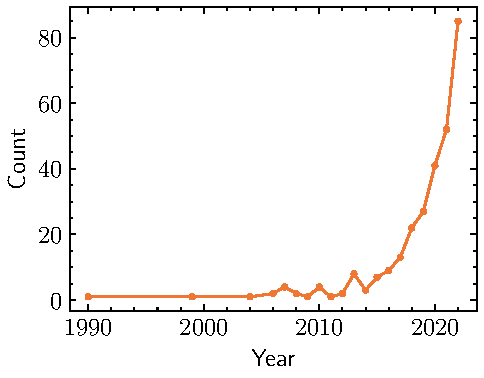
\includegraphics{pictures/scopus.pdf}
    \caption{Number of scientific publications (journal and conference papers) in English language containing the terms "learning" and "MILP" in their title, abstract or keywords. Source: SCOPUS}
    \label{fig:scopus-trend}
\end{figure}

\subsection*{Objectives}\label{chap:objectives}
\addcontentsline{toc}{section}{Objectives}

In the topic of this dissertation, three research questions are of fundamental importance in the development of heuristic approaches:
\begin{itemize}
    \item How to design deep learning models to provide candidate solutions for instances of an MILP problem?
    \item Which supervised learning techniques are most effective for training solution prediction models for primal heuristics? And
    \item How to incorporate solution prediction models in primal heuristics?
\end{itemize}
Targeting these questions, this dissertation aims \emph{to evaluate primal heuristics for MILP problems based on solution prediction models trained with supervised learning techniques}.
This goal is broken down into three objectives:
\begin{itemize}
    \item Analyze the literature on supervised learning solution prediction models for MILP problems, including model architectures, supervised learning algorithms, and learning-based primal heuristics;
    \item Develop learning-based primal heuristics for a realistic application based on the most promising techniques found in the literature; and
    \item Evaluate the techniques for learning-based heuristics with respect to the empirical performance in a realistic application and the theoretical guarantees provided by each.
\end{itemize}
The achievement of these objectives will result in the two major contributions of this work to the research community.

% \phantompart


	\part{Background}\label{background}

	
% The \phantomsection command is needed to create a link to a place in the document that is not a
% figure, equation, table, section, subsection, chapter, etc.
% https://tex.stackexchange.com/questions/44088/when-do-i-need-to-invoke-phantomsection
\phantomsection

\chapter{Integer Programming}\label{chap:integer-programming}


Integer Programming (IP), a subset of mathematical programming, addresses optimization problems where decision variables are required to take on integer values.
Specifically, mixed-integer linear programming (MILP) extends this concept by encompassing the assumption that for each possible discrete decision, a (continuous) linear program has to be solved.
The complexity of MILP problems often necessitates sophisticated solution methods to find optimal or near-optimal solutions.
This chapter provides an overview of MILP problem-solving techniques, ranging from exact methods like the branch-and-bound algorithm to approaches to provide approximate solutions, such as heuristics and matheuristics.
Through these methodologies, the groundwork is laid for the subsequent discussion on deep learning-based primal heuristics, which aim to enhance the efficiency of MILP problem solving.

\section{Integer and Combinatorial Optimization}

A solution for an integer and combinatorial optimization problem is the maximum or minimum value of a multivariate function that respects a series of inequality and equality constraints and integrality restrictions on some or all variables~\cite{nemhauserIntegerCombinatorialOptimization1999}.
It is not difficult to see that integer and combinatorial optimization encompasses a wide range of problems of practical utility.
Examples include train scheduling, airline crew scheduling, production planning, electricity generation planning, and cutting problems~\cite{wolseyIntegerProgramming1998}.

Mathematical programming is a language naturally suitable to formulate integer and combinatorial optimization problems, for example, in the form
\begin{equation}\label{eq:general-ip}\tag{IP}
    \begin{split}
	\min_{\bm{y}} \quad & f\left( \bm{y} \right) \\
	\textrm{s.t.} \quad & \bm{g}\left( \bm{y} \right) \le \bm{0} \\
	  & \bm{y} \in \Z^{n}\times \R^{p}
    ,\end{split}
\end{equation}
where $\bm{y}$ are the \emph{decision variables}, of which $y_1,\ldots,y_n$ are integer variables and $y_{n+1},\ldots,y_{n+p}$ are continuous variables.
Furthermore, $\bm{g}: \Z^{n}\times \R^{p} \longrightarrow \R^{m}$,  and $\bm{0}$ is a null vector of dimension $m$.
Note that maximizing a function is equivalent to minimizing its negative, and an equality constraint can be represented by two inequalities, which renders \eqref{eq:general-ip} a complete formulation.

For an integer program formulated as in \eqref{eq:general-ip}, the set \[
Y=\left\{ \bm{y}\in \Z^{n}\times \R^{p}: \bm{g}\left( \bm{y} \right) \le \bm{0}\right\} 
\] is named the \emph{feasible region} of the problem, and a vector $\bm{y}\in Y$ is a \emph{feasible solution}.
A feasible solution $\bm{y}^{*}\in Y$ is \emph{optimal} if, and only if, there is no other feasible solution with a lower value of the \emph{objective function} $f: \Z^{n}\times \R^{p} \longrightarrow \R$, i.e., $\bm{y}^{*}$ is optimal $\iff f(\bm{y}^{*}) \le f(\bm{y}) ,\,\forall \bm{y}\in Y$.

Note that even if a problem is feasible ($Y\neq \varnothing$), it may not have an optimal solution, e.g., if the feasible region is unbounded and the objective function has no global minimum.
Furthermore, if an optimal solution exists, it may no be unique.
% TODO: show how a problem may have no optimal solution even if with bounded feasible region. see Nemhauser, I.4.6

Beyond the practical applications of integer programming, its computational complexity renders it an important theoretical model.
It is easy to see that integer programming is an NP-hard problem~\cite{nemhauserIntegerCombinatorialOptimization1999}.
In fact, one of Karp's 21 NP-complete problems~\cite{karpReducibilityCombinatorialProblems1972} is a special case of integer programming with no objective function (constraint satisfaction problem) and solely binary variables.

\section{Mixed-Integer Linear Programs}\label{sec:milp-definition}

MILP is a subset of IP in which the objective and the constraints are all linear functions and the problem requires integer and continuous variables.
Formally, an MILP can be formulated as 
\begin{equation}\label{eq:general-milp}\tag{MILP}
\begin{split}
    \min_{\bm{y}} \quad & \bm{c}^{T}\bm{y} \\
    \textrm{s.t.} \quad & A\bm{y} \le \bm{b} \\
	  & \bm{y} \in \Z^{n}\times \R^{p} ,\end{split} \end{equation} where
	  $A\in \R^{m\times (n+p)}$ is the constraint matrix, $\bm{b}\in
	  \R^{m}$ is the right-hand side vector, and $\bm{c}\in \R^{n+p}$ is
	  the cost vector.  An \emph{instance} of an MILP problem is specified
	  by a tuple  $\left( \bm{c},\bm{b},A,n \right)$.

	  The significance of this class of problems has already been
	  recognized by \citeonline{dantzigSignificanceSolvingLinear1960}.
	  Many well-known problems can be formulated through MILP, such as the
	  Traveling Salesperson Problem (TSP) and the map coloring problem.
	  Furthermore, continuous nonlinear functions can be approximated to
	  arbitrary quality by piecewise linear functions, which admit an MILP
	  formulation~\cite{camponogaraModelsAlgorithmsOptimal2015}.  In other
	  words, MILP is a powerful tool for approximating optimization
	  problems with continuous nonlinearities.

	  \section{Solving MILP Problems}

	  % TODO: solving MILP is hard, in fact, it is NP-hard, as seen Karp's 
	  Although MILP offers powerful models for a wide range of problems,
	  solving such problems is unarguably hard.  In fact, the NP-complete
	  problem formulated by
	  \citeonline{karpReducibilityCombinatorialProblems1972} only contains
	  linear terms, which renders it a special case of MILP and, thus,
	  assuming P$\neq$NP, classifies MILP problems as NP-hard.  However,
	  despite the intractable nature, there are efficient and reliable
	  algorithms and software solutions for the computation of optimal and
	  approximate solutions to MILP
	  problems~\cite{bengioMachineLearningCombinatorial2021}.  Furthermore,
	  the applications of MILP often require high-quality solutions in a
	  limited time, which motivate the development of heuristic approaches,
	  i.e., approaches that trade optimality (or feasibility) guarantees
	  for a tractable running time.

	  \subsection{The Branch-and-Bound Algorithm}

	  The branch-and-bound algorithm follows a divide-and-conquer approach.
	  An MILP problem is divided into smaller, easier problems, and the
	  solution to these problems is combined such that a solution to the
	  original problem is found~\cite{wolseyIntegerProgramming1998}.

	  An MILP problem is divided by decomposing its feasible region.  Given
	  a problem $P$ as in \eqref{eq:general-milp} with feasible region
	  $Y=\{\bm{y}\in \Z^{n}\times \R^{p}: A\bm{y}\le \bm{b}\}$, a
	  decomposition of its feasible region $Y_1,\ldots,Y_K$ is such that
	  $Y=Y_1\cup \cdots\cup Y_K$.
In this context, a subproblem is
\begin{equation}\label{eq:milp-subproblem}
\begin{split}
    P^{(k)} : \min_{\bm{y}} \quad & \bm{c}^{T}\bm{y} \\
    \textrm{s.t.} \quad & \bm{y}\in Y_k
,\end{split}
\end{equation}
for which $\bm{y}^{k}$ is the optimal solution and $z^{k}=\bm{c}^{T}\bm{y}^{k}$ is the optimal cost.
If the $k$-th subproblem is infeasible, it is assumed that $z^{k}=\infty$.
If $k^{*}= \arg\min_k z^{k}$, then $z^{k^*}$ is the optimal value of the MILP problem $P$ and $\bm{y}^{k^*}$ is its optimal solution.

A decomposition is useful for a divide-and-conquer approach if the resulting subproblems are significantly easier to solve than the original problem.
One way to achieve this is by decomposing the feasible region on the values for the integer variables.
If this decomposition strategy is performed recursively until all integer variables have only one feasible assignment in each $Y_k$, then each $P^{(k)}$ is an LP problem, which allows us to compute, for each $k$, the optimal solution in polynomial time.
For example, consider an MILP problem with 3 binary variables, i.e., with $Y\subseteq \{0,1\}^{3}\times \R^{p}$.
By recursively decomposing $Y$ on the possible assignments for each binary variable, the tree structure of Fig.~\ref{fig:binary-MILP-tree-example} could be assembled.
% Note that a decomposition can be progressively generated by exploring the tree, e.g., $X=X_1\cup X_2\cup X_3\cup X_4$, $X=X_1\cup X_2\cup X_3\cup X_{4, 1}\cup X_{4,2}$, \ldots, $X=X_{1,1}\cup X_{1,2}\cup X_{2,1}\cup \ldots\cup X_{4,2}$.
% Note that $X_{1,2}$ and $X_{4,2}$ are empty sets, i.e., the associated subproblems are infeasible.

\begin{figure}[h]
    \centering
    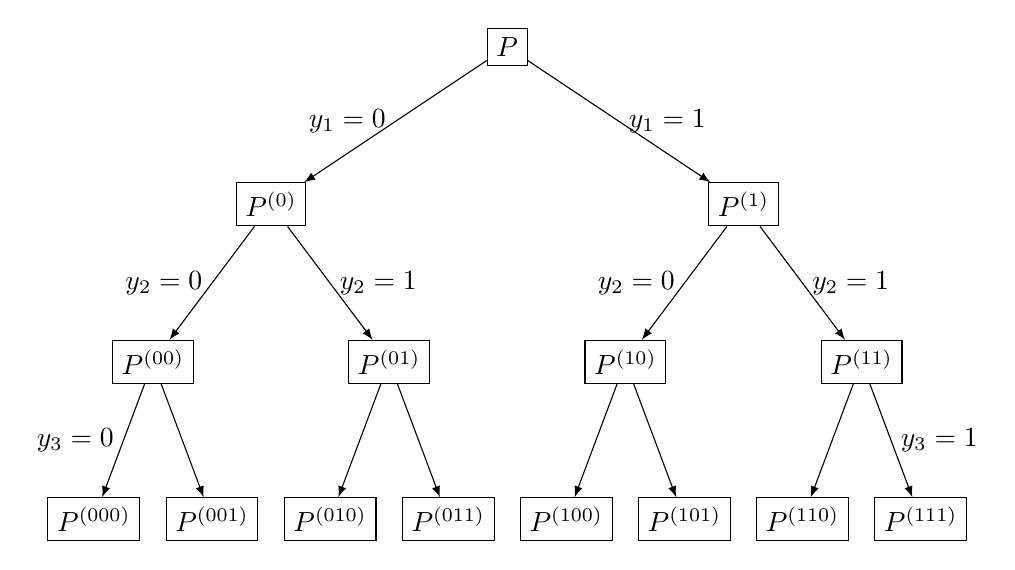
\begin{tikzpicture}[every child node/.style={rectangle,draw},level 1/.style={sibling distance=6cm},level 2/.style={sibling distance=3cm},level 3/.style={sibling distance=1.5cm}, level distance = 2cm,edge from parent/.style={draw,-latex}]
        \node[rectangle,draw] (Y) {$P$} 
	    child { node {$P^{(0)}$}
        	child { node {$P^{(00)}$}
		    child { node {$P^{(000)}$} edge from parent node [midway,left] {$y_3=0$} }
		    child { node {$P^{(001)}$} }
		    edge from parent node [midway,left] {$y_2=0$}
		}
        	child { node {$P^{(01)}$}
		    child { node {$P^{(010)}$} }
		    child { node {$P^{(011)}$} }
		    edge from parent node [midway,right] {$y_2=1$}
		}
        	edge from parent node [midway,left] {$y_1=0$}
            }
            child { node {$P^{(1)}$}
        	child { node {$P^{(10)}$}
		    child { node {$P^{(100)}$} }
		    child { node {$P^{(101)}$} }
		    edge from parent node [midway,left] {$y_2=0$}
		}
        	child { node {$P^{(11)}$}
		    child { node {$P^{(110)}$} edge from parent }
		    child { node {$P^{(111)}$} edge from parent node [midway,right] {$y_3=1$} }
		    edge from parent node [midway,right] {$y_2=1$}
		}
        	edge from parent node [midway,right] {$y_1=1$}
            }
            ;
	%\node[left = of x2] (x2_label) {$x_2=$};
	%\node at (x2_label |- x1) {$x_1=$};
	% \node[left = of x1 -| x2] {$x_1=$};
    \end{tikzpicture}
    \caption{Complete decomposition of an MILP problem on its 3 binary variables. Nodes are annotated with the associated subproblems. Assuming that the problem has no other integer variables, the subproblems at the leaf nodes are LP problems.}
    \label{fig:binary-MILP-tree-example}
\end{figure}

Unfortunately, completely decomposing an MILP problem through the integer variable assignments is only possible for very small, bounded problems.
If the problem is unbounded in the integer variables, the complete decomposition would result in an infinite recursion.
Furthermore, the number of leaf nodes grows exponentially with the size of the problem\footnotemark.
\footnotetext{In this context, the size of the problem is measured as the number of binary variables that the equivalent reformulation as a binary MILP would contain. The number of leaf nodes grows exponentially (with base 2) with respect to the number of such binary variables.}

The branch-and-bound algorithm follows an implicit approach that uses upper and lower bounds to avoid indefinitely dividing subsets from the decomposition.
Let $P$ be an MILP problem formulated as in \eqref{eq:general-milp} and $Y_1,\ldots,Y_K$ be a decomposition of the feasible region $Y$.
If $\underline{y}^{k}$ and $\overline{y}^{k}$ are lower and upper bounds to $z^{k}$ (optimum cost of $P^{(k)}$), for every $k=1,\ldots,K$, then, it is true that \[
\min_k \underline{y}^{k} \le z \le \min_k \overline{y}^{k}
,\] 
where $z$ is the optimum cost of $P$.
In other words, we can compute bounds of the root problem as $\underline{y}\gets \min_k \underline{y}^{k}$ and $\overline{y}\gets \min_k \overline{y}^{k}$.
Finally, if $\underline{y}^{k} \ge \overline{y}$ for a given $k$, then the optimal solution of $P^{(k)}$ will not be an optimal solution of $P$, because it is guaranteed that another subproblem has a better feasible solution.
In other words, even if the optimal solution of $P^{(k)}$ is unknown, it is possible to disregard $Y_k$ in the decomposition, i.e., $Y_k$ does not need to be further subdivided. 

For example, let $P$ be an MILP problem and $Y=Y_1\cup Y_2$ be a decomposition such that $Y_1=\{\bm{y}\in Y: y_1 \le 2\}$ and $Y_2=\{\bm{y}\in Y: y_1 \ge 3\}$.
Suppose that the LP relaxations\footnote{The linear programming problem obtained by ignoring the integrality constraints of an MILP is called its \emph{LP relaxation}.} of $P^{(1)}$ and $P^{(2)}$ were solved to optimality, giving lower bounds $\underline{y}^1=20$ and $\underline{y}^{2}=15$, and that a feasible solution to $P$ is known in $Y_2$ such that the upper bound $\overline{y}^{2}=17$ is known.
Fig.~\ref{fig:pruning-example-milp} illustrates the decomposition along with respective bounds in the form of a tree.
Because the lower bound of $P^{(1)}$ is greater than the original problem's upper bound (as $\overline{y}=\min_k \overline{y}^{k}$), the optimal solution is definitely not in $Y_1$, so this set is ignored in the decomposition and not further refined.

\begin{figure}[h]
    \centering
    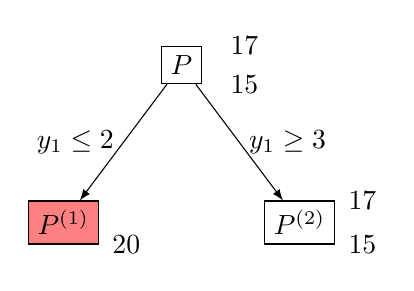
\begin{tikzpicture}[every child node/.style={rectangle,draw},level 1/.style={sibling distance=3cm}, level distance = 2cm,edge from parent/.style={draw,-latex}]
        \node[rectangle,draw] (P) {$P$} 
	    child { node[fill=red!50] (P1) {$P^{(1)}$}
        	edge from parent node [midway,left] (z1) {$y_1\le 2$}
            }
            child { node (P2) {$P^{(2)}$}
        	edge from parent node [midway,right] {$y_1 \ge 3$}
            }
            ;
	%\node[above = 0cm of P] {$15\le z\le 17$} ;
	\node[right = 0.5cm of P.south] {$15$} ;
	\node[right = 0.5cm of P.north] {$17$} ;
	\node[right = 0.5cm of P1.south] {$20$} ;
	\node[right = 0.5cm of P2.north] {$17$} ;
	\node[right = 0.5cm of P2.south] {$15$} ;
	%\node[left = of x2] (x2_label) {$x_2=$};
	%\node at (x2_label |- x1) {$x_1=$};
	% \node[left = of x1 -| x2] {$x_1=$};
    \end{tikzpicture}
    \caption{Example of pruning the decomposition of an MILP problem based on known bounds. The lower (resp. upper) bounds of each (sub)problem are annotated at the bottom (resp. top) right of each node. The node associated to set $Y_1$ is painted red to indicate it is pruned based on the bounds of the root problem, which are updated based on the bounds from $P^{(2)}$.}
    \label{fig:pruning-example-milp}
\end{figure}

Because of the usual tree representation, the operation of disregarding a set in the decomposition is often called \emph{pruning}.
Three basic rules can be listed that lead to pruning of the branch associated to set $Y_k$:
\begin{itemize}
    \item[Optimality] Subproblem $P^{(k)}$ was solved to optimality (e.g., through its LP relaxation having an optimal solution that respects the integrality constraints);
    \item[Bound] The associated lower bound is higher than the upper bound of the root problem ($\underline{y}^{k}\ge \overline{y}$);
    \item[Infeasibility] $Y_k = \varnothing$.
\end{itemize}


The two key components of a branch-and-bound algorithm are the pruning system based on \emph{bounds}, as discussed above, and the rules for subdividing the sets in the decomposition, or \emph{branching}.
A simple strategy for branching is to choose an integer variable that has taken a fractional value in the optimal solution to the LP relaxation and split the problem on this factional value.
For example, let $Y_k$ be a set in the decomposition of an MILP problem, and $P^{(k)}$ be the associated subproblem.
Let $\widetilde{\bm{y}}^{k}$ be the solution to the LP relaxation of $P^{(k)}$, and suppose that the integer variable $y_3$ takes value $3.67$ in $\widetilde{\bm{y}}^{k}$.
Following the proposed branching strategy on $y_3$, the sets $Y_{k_1}$ and $Y_{k_2}$ would be created such that \[
Y_{k_1} = \left\{ \bm{y} \in Y_k : y_3 \le 3 \right\} ,\, Y_{k_2} = \left\{ \bm{y}\in Y_k : y_3 \ge 4 \right\} 
,\] and the set $Y_k$ would then be replaced in the decomposition by these two new sets.
Fig.~\ref{fig:branching-example} illustrates this example.

\begin{figure}[h]
    \centering
    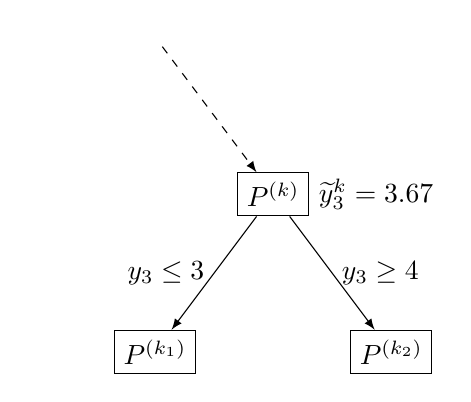
\begin{tikzpicture}[every child node/.style={rectangle,draw},level 1/.style={sibling distance=3cm}, level distance = 2cm,edge from parent/.style={draw,-latex}]
        \node (P) {} 
	    child { node[draw=none] (P1) {}
        	edge from parent [draw=none]
            }
            child { node (Pk) {$P^{(k)}$}
		child { node [solid] (Pk1) {$P^{(k_1)}$}
		    edge from parent [solid] node [midway,left] (z1) {$y_3\le 3$}
		}
		child { node [solid] (Pk2) {$P^{(k_2)}$}
		    edge from parent [solid] node [midway,right] (z2) {$y_3\ge 4$}
		}
        	edge from parent [dashed] 
            }
            ;
	\node[right = 0cm of Pk.east] {$\widetilde{y}^{k}_3 = 3.67$} ;
    \end{tikzpicture}
    \caption{Example of branching on a given set $Y_k$ which is part of the decomposition of an MILP problem. Only the relevant part of the tree is illustrated (indicated by the dashed arrow). The optimum value of $y_3$ (the selected integer variable for branching) in the LP relaxation of $P^{(k)}$ is annotated next to the appropriated node.}
    \label{fig:branching-example}
\end{figure}

Note that by branching on the fractional value of an integer variable in the optimal solution to the LP relaxation, the optimal solution of the LP relaxation becomes infeasible in the LP relaxations of the new sets\footnote{This is true unless there are degeneracies such as multiple solutions in the LP relaxation}.
Therefore, after branching, the best lower bound will necessarily increase.
Using the example above to make this result tangible, it is possible to state that $\widetilde{\bm{y}}^{k}$ is infeasible for the LP relaxations of both $P^{(k_1)}$ and $P^{(k_2)}$.
Therefore, $\max\{\underline{y}^{k_1},\underline{y}^{k_2}\} > \underline{y}^{k}$.

%As an example, take the MILP problem\footnote{Example taken from \citeonline{vanderbeiLinearProgrammingFoundations1998}, Ch. 22.5.}
%\begin{align*}
%    \min_{\bm{x}} \quad & -17 x_1 - 12x_2 \\
%    \textrm{s.t.} \quad & 10x_1 + 7x_2 \le 40 \\
%      & x_1+x_2\le 5 \\
%      & \bm{x} \in \Z_+^2
%.\end{align*}

There are many more intricate details to the construction of a branch-and-bound algorithm, such as the strategy for choosing a set in the decomposition to refine, the amount of information from each node of the tree to be stored, efficient reoptimization, and computing the bounds using the dual.
The reader is pointed to \citeonline{wolseyIntegerProgramming1998} and \citeonline{vanderbeiLinearProgrammingFoundations1998} for advanced topics and detailed examples.


\subsection{Heuristics}\label{sec:heuristics}

Although branch-and-bound provides an efficient algorithmic approach to solve an MILP problem, there is no guarantee that it will find a feasible (let alone an optimal) solution considering the NP-hardness of the problem.
The development of heuristic or approximation algorithms is justified in many ways, as can be seen in \citeonline{wolseyIntegerProgramming1998}, Chapter 12.
The major one, for this work, is from practical applications with significant running time cost.
In simple terms, such applications require good solutions quickly, rather than optimal solutions in an unknown time-horizon.

Heuristic algorithms are an umbrella term that encompass several different algorithms with different characteristics.
Overall, distinguishing features of heuristics are on the feasibility and optimality of the solutions returned.
For feasibility, it is important to know if there are feasibility guarantees on the heuristic solution or, at least, an expectation on how often the heuristic will return infeasible solutions.
Similarly, it is relevant to understand whether the solutions provided are guaranteed to be within a limited distance (in terms of the objective function) of the optimal solutions, or if there is an expected value for such distance. 
Such heuristics with quality guarantees are referred to as approximation algorithms in the technical literature

Common examples of heuristic algorithms are greedy algorithms and local search approaches~\cite{nemhauserIntegerCombinatorialOptimization1999,wolseyIntegerProgramming1998}.
Greedy heuristics construct the solution incrementally by selecting, at each step, the alternative that best improves the objective function.
Take the Symmetric TSP (STSP) as an example.
A greedy heuristic for such problem could be to add to the solution the edge with the smallest cost.
Note that this greedy heuristic will always return a feasible solution, although it is not expected that the solution will be close to optimal.

Local search algorithms take a feasible solution and try to improve the objective function by performing only limited changes.
Given a complete tour (feasible solution) for the STSP, a small deviation can be achieved by removing two non-consecutive edges that are part of the solution and adding two \emph{different} edges that reconnect the two disjoint paths.
This way, a new tour will be achieved that differs from the original by two edges.
In other words, such local search is limited to a 2-neighborhood of the original tour.

A general heuristic (or metaheuristic) algorithm for MILP problems is \emph{diving}~\cite{fischettiHeuristicsMixedInteger2011}.
Diving methods solve the LP relaxation, fix integer variables that assume fractional values, and update the LP relaxation.
This process is repeated until there are no more integer variables to be fixed.
It is often called diving because it is equivalent to quickly navigating to a leaf node in a branch-and-bound tree.

Recently, heuristics based on machine learning models have been proposed~\cite{bengioMachineLearningCombinatorial2021}.
This will be discussed in Section~\ref{sec:learning-based-heuristics}.

\subsubsection{Matheuristics}\label{sec:matheuristics}

Matheuristics is the name given to heuristic algorithms that use a mathematical programming model at its core.
In fact, the diving algorithm introduced above can be seen as a form of matheuristic.
In this section, however, the focus is on algorithms that actively optimize mathematical programming models.
Relaxation induced neighborhood search (RINS)~\cite{maniezzoMatheuristicsAlgorithmsImplementations2021} exemplifies the distinction intended in this chapter.

The RINS algorithm aims to improve a feasible solution by solving a smaller MILP problem. 
A neighborhood around a feasible solution is defined by fixing the values of some integer variables.
The search on this neighborhood is performed by adding the variable fixing constraints to the original problem, effectively reducing its feasible region.
Let $P$ be an MILP problem as in \eqref{eq:general-milp}, $\bm{y}^{h}$ be a feasible solution, and $\widetilde{\bm{y}}$ the solution to the LP relaxation of $P$.
Let $J = \{j = 1,\ldots,n : y_j^{h} = \widetilde{y}_j\}$ be the index set of integer variables to fix.
Then, the sub-MILP problem
\begin{align*}
    \min_{\bm{y}} \quad & \bm{c}^{T}\bm{y} \\
    \textrm{s.t.} \quad & A\bm{y}\le \bm{b} \\
      & y_j = y_j^{h}, \forall j \in J \\
      & \bm{y}\in \Z^{n}\times \R^{p}
\end{align*}
can be solved, e.g., using branch-and-bound.
Note that all integer variables that assume the same value in the feasible solution and in the solution to the LP relaxation are fixed, thus, reducing the search space, but abdicating from optimality guarantees.

As the RINS example above illustrates, a mathematical programming model plays a central role in a matheuristic~\cite{fischettiMatheuristics2016}.
Because of their flexibility, matheuristics are also used within branch-and-bound algorithms, e.g., to find tighter bounds and accelerate the time to reach the first feasible solution~\cite{fischettiMatheuristics2016,maniezzoMatheuristicsAlgorithmsImplementations2021}.

\subsubsection{Performance analysis}

The performance analysis of heuristic algorithms depends on the instances of interest.
To better formalize this idea, let us write
\begin{align*}
    P(I): \min_{\bm{y}} \quad & \bm{c}_I^{T}\bm{y} \\
    \textrm{s.t.} \quad & A_I\bm{y} \le \bm{b}_I \\
      & \bm{y}\in \Z^{n_I}\times \R^{p_I}
,\end{align*}
for all instances $I\in \mathcal{I}$.
The set $\mathcal{I}$ contains all instances of the MILP problem of interest, e.g., all TSPs, TSPs within a given country with all possible edge weights, course scheduling for a given university for varying student interest, or energy system optimization problems for a multi-modal power plant under different weather conditions.
Using this notation, it is possible to say that the performance of the heuristic can be analyzed from the set $\mathcal{I}$.

A possible evaluation is to perform a worst-case analysis of the heuristic.
The essential idea of a worst-case analysis is to determine the maximum deviation between the optimum objective value and the objective value of the heuristic solution. 
Let $z(I)$ be the optimum objective value of instance $I\in \mathcal{I}$, and $z_H(I)$ be the objective value of the solution provided by a heuristic $H$.
The worst-case performance is, then,
\begin{equation}
    \begin{split}
	\max_{I\in \mathcal{I}} \quad& |z(I) - z_H(I)| \\
	\textrm{s.t.} \quad& Y_I \neq \varnothing
    ,\end{split}
\end{equation}
where $Y_I$ is the feasible region of instance $I$.

Not always, however, the worst-case performance can be determined analytically.
A performance estimate can be defined in such cases.
Let $\mathcal{P}$ be a probability distribution over $\mathcal{I}$.
The expected performance of a heuristic can be defined as \[
    \mathbb{E}_{I\sim \mathcal{P}} |z(I) - z_H(I)|
,\] which can be approximated by Monte Carlo sampling.




	%% chapters/chapter_2.tex
%%
%% Copyright 2017 Evandro Coan
%% Copyright 2012-2014 by abnTeX2 group at http://abntex2.googlecode.com/
%%
%% This work may be distributed and/or modified under the
%% conditions of the LaTeX Project Public License, either version 1.3
%% of this license or (at your option) any later version.
%% The latest version of this license is in
%%   http://www.latex-project.org/lppl.txt
%% and version 1.3 or later is part of all distributions of LaTeX
%% version 2005/12/01 or later.
%%
%% This work has the LPPL maintenance status `maintained'.
%%
%% The Current Maintainer of this work is the Evandro Coan.
%%
%% The last Maintainer of this work was the abnTeX2 team, led
%% by Lauro César Araujo. Further information are available on
%% https://www.abntex.net.br/
%%
%% This work consists of a bunch of files. But originally there were 2 files
%% which are renamed as follows:
%% Deleted the `abntex2-modelo-img-marca.pdf`
%% Renamed the `abntex2-modelo-include-comandos.tex, v-1.9.2 laurocesar` to `chapters/chapter_1.tex`
%%
% ---
% Este capítulo, utilizado por diferentes exemplos do abnTeX2, ilustra o uso de
% comandos do abnTeX2 e de LaTeX.
% ---

% The \phantomsection command is needed to create a link to a place in the document that is not a
% figure, equation, table, section, subsection, chapter, etc.
% https://tex.stackexchange.com/questions/44088/when-do-i-need-to-invoke-phantomsection
\phantomsection

% https://tex.stackexchange.com/questions/5076/is-it-possible-to-keep-my-translation-together-with-original-text
\chapter{Deep Learning}\label{chap:deep-learning}

The advent of deep learning has revolutionized numerous fields, offering unprecedented capabilities in pattern recognition, decision-making, and problem-solving~\cite{Goodfellow-et-al-2016}.
In the realm of combinatorial optimization, particularly MILP, traditional methods often encounter computational bottlenecks when solving large-scale instances.
However, recent strides in deep learning have opened up exciting avenues for developing effective primal heuristics.
This chapter delves into the background of deep learning, focusing on the fundamental principles of supervised learning and neural network architectures.
The understanding of such concepts is essential for exploring the design and implementation of deep-learning-based solution prediction models tailored to MILP instances.


\section{Supervised Learning}

Supervised learning can be seen as the problem of finding a function that best associates inputs $x$ to outputs $y$ given a \emph{training set} with finitely many examples of such inputs and outputs~\cite{Goodfellow-et-al-2016}.
Although the machine learning (ML) area has attracted plenty of attention in the last decade, this learning problem is not new.
In fact, the core concepts were already established in the 1960s and 1970s~\cite{vapnikNatureStatisticalLearning2000}.
This section's approach to supervised learning will be that of statistical learning theory, based on \citeonline{vapnikNatureStatisticalLearning2000}, but with a more modern notation, derived from pattern recognition~\cite{bishopPatternRecognitionMachine2006,hastieElementsStatisticalLearning2009}.

\subsection{Supervised learning algorithm}

Supervised learning will be defined here as a problem of estimating a function that minimizes the risk.
Let $\mathcal{X}$ and $\mathcal{Y}$ be the input and output space, and $\mathcal{P}$ be a joint probability distribution over $\mathcal{X}\times \mathcal{Y}$.
To evaluate a function $f: \mathcal{X} \longrightarrow \mathcal{Y}$ with respect to its capacity to perform the right association between an input $x\in \mathcal{X}$ and an output $y\in \mathcal{Y}$, one measure's the discrepancy, or the \emph{loss}, $\ell(y,f(x))$.
In this context, the \emph{risk} associated to $f$ over the joint distribution $\mathcal{P}$ is the expected value of the loss function, or \[
    R(\mathcal{P},f) = \int_{\mathcal{X}\times \mathcal{Y}} \ell(y,f(x))\mathcal{P}(x,y)
    %R(f) = \mathbb{E}_{(x,y)\sim \mathcal{P}} \ell(y,f(x))
.\] 

The machine learning paradigm is that the joint probability function is fixed, but unknown, and one only has access to a finite number of samples~\cite{vapnikNatureStatisticalLearning2000}.
This idea is best represented through a \emph{dataset}, which is a finite set $\mathcal{D}$ of independent and identically distributed (i.i.d.) samples drawn according to $\mathcal{P}$.
In this context, the \emph{empirical risk} associated to a function $f$ over a dataset $\mathcal{D}$ is \[
    R_\textrm{emp}(\mathcal{D},f) = \frac{1}{|\mathcal{D}|} \sum_{(x,y)\in \mathcal{D}} \ell(y, f(x))
.\]

In this work, it is considered that the function to be estimated is chosen from a \emph{parametric model}\footnotemark, which is a family of functions $f_\theta: \mathcal{X} \longrightarrow \mathcal{Y}$ defined over a parameter space $\Theta \ni \theta$.
\footnotetext{This is in contrast to non-parametric models, whose functions' parameters are defined in terms of the dataset~\cite{murphyMachineLearningProbabilistic2013}.}
The problem then becomes that of finding a parameter vector that minimizes the empirical risk from a dataset $\mathcal{D}$, or \emph{fitting} a model to a dataset, denoted
\begin{equation}\label{eq:cost-minimization}
    \min_{\theta \in  \Theta} \mathcal{L}(\theta)
,\end{equation}
where
\begin{equation}\label{eq:cost-function}
    \mathcal{L}(\theta) = \frac{1}{|\mathcal{D}|} \sum_{(x,y)\in \mathcal{D}} \ell(y, f_\theta(x))
\end{equation}
is an alternate, commonly found notation for the empirical risk, which often carries the name \emph{cost function}~\cite{murphyMachineLearningProbabilistic2013,Goodfellow-et-al-2016}.
Both "empirical risk" and "cost function" will be used interchangeably throughout this dissertation, although the former has a stronger connection to learning theory, while the latter is more related to practical matters.

A supervised learning algorithm is essentially an algorithm to optimize a cost function given a model and a dataset.
In fact, it is possible to define a supervised learning algorithm as a simple recipe: ``combine a specification of a dataset, a cost function, an optimization procedure and a model''~\cite{Goodfellow-et-al-2016}.
Many different algorithms exist that are suitable for different components of this recipe.
For example, there are algorithms particular to decision tree models~\cite{breimanClassificationRegressionTrees2017}.
The least squares algorithm (used in the example of Section~\ref{sec:generalization-overfitting}) can be seen as a supervised learning algorithm for polynomial models given and the squared error loss function.

\subsection{Generalization and overfitting}\label{sec:generalization-overfitting}

Blindly minimizing the empirical risk can lead to a problem named \emph{overfitting}.
Overfitting happens when the empirical risk does not reflect the true risk, that is, when a function is \emph{fit} for the dataset, but not for the underlying data distribution.

This concept is best understood through an example.
Suppose $\mathcal{X},\mathcal{Y}\subseteq\R$ and that a dataset $\mathcal{D}$ with 40 i.i.d. samples is obtained such as illustrated in Fig.~\ref{fig:overfitting-example}.
It is desired to find a function that minimizes the risk measured through the squared error loss \[
    \ell(y,f(x)) = (y-f(x))^2
.\] 
The models $f^{(1)},f^{(2)},f^{(3)}$ are polynomials of degree 1, 3, and 15, whose parameters are the weights of the polynomials.
These models are adjusted using least squares algorithm, resulting in parameter vectors $\theta_1^*,\theta_2^*,\theta_3^*$ that achieve a global minimum of the empirical risk with their respective models.
The performance of these models is illustrated in Fig.~\ref{fig:overfitting-example}.

Note that model $f^{(3)}$ achieves the lowest empirical risk on $\mathcal{D}$.
However, $f^{(2)}$ is the one that seems to best associates inputs to outputs, considering a visual intuition of the underlying data distribution.
One could say that $f^{(3)}$ is \emph{too complex} for the underlying distribution, which leads to it being more tightly adjusted to the noise present in the dataset rather than on the underlying data distribution~\cite{murphyMachineLearningProbabilistic2013}.
On the other hand of the spectrum is the $f^{(1)}$ model, which is not complex enough to model the desired behavior.
While $f^{(3)}$ is overfitting the data, $f^{(1)}$ is underfitting it.

\begin{figure}[h]
    \centering
    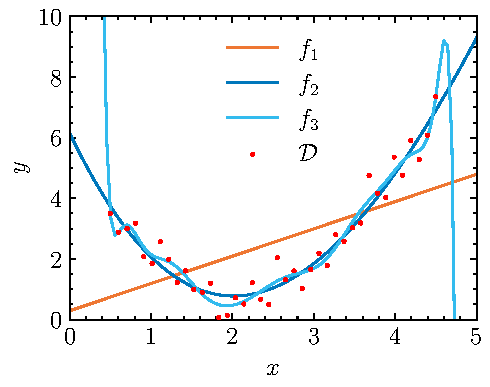
\includegraphics{pictures/overfitting.pdf}
    \caption{Example of overfitting. The three models shown ($f^{(1)},f^{(2)},f^{(3)}$) are families of polynomials of degree 1, 3 and 10, respectively. The optimal parameter vectors $\theta_1^*,\theta_2^*$ and $\theta_3^*$ were optimized to the dataset $\mathcal{D}$ using a least squares algorithm. The empirical risks are $\mathcal{L}(\theta_1^*)=79.67$, $\mathcal{L}(\theta_2^*)=7.64$, and $\mathcal{L}(\theta_3^*)=5.48$.}
    \label{fig:overfitting-example}
\end{figure}

The level of overfitting that a function $f$ presents could be determined through the \emph{generalization gap}, which is the difference between the empirical risk and the true risk $R(\mathcal{P},f) - R_\textrm{emp}(\mathcal{D},f)$~\cite{murphyMachineLearningProbabilistic2013}.
More specifically, a function can be said to overfit the dataset if it has a high generalization gap.
As the underlying distribution $\mathcal{P}$ is not known, the generalization gap is approximated by \emph{splitting} the dataset $\mathcal{D}$ into a training set $\mathcal{D}_\textrm{train}$ and a test set $\mathcal{D}_\textrm{test}$.
The idea is that the parameters of the model are adjusted according to the empirical risk of $\mathcal{D}_\textrm{train}$, while $\mathcal{D}_\textrm{test}$ is reserved for estimating the true risk, also called \emph{generalization error}.
This way, the resulting function cannot be overfitted to $\mathcal{D}_\textrm{test}$, which is kept as an untouched source of information of the underlying distribution.
Finally, the generalization gap can be estimated as  \[
    R_\textrm{emp}(\mathcal{D}_\textrm{test},f) - R_\textrm{emp}(\mathcal{D}_\textrm{train},f)
.\] 

\subsection{Hyperparameter tuning}

Hyperparameters are the settings that modify the behavior of a supervised learning algorithm~\cite{Goodfellow-et-al-2016}.
These hyperparameters can be configurations of the optimization algorithm or parameters of the model that are not adjusted by the algorithm.
Hyperparameter adjustment is impactful both in the runtime of the algorithm, and in the quality of the function returned.

In the polynomial fitting example above (illustrated in Fig.~\ref{fig:overfitting-example}), the polynomial degree is a hyperparameter.
Different values for this hyperparameter result in totally different parameter spaces $\Theta$ over which the optimizer will search for a risk minimizer.
If a ridge regression algorithm is used instead of the least squares to find the optimal function, then a hyperparameter is the weight of the $\ell_2$-norm of $\theta$.
Such hyperparameter does not alter the function space associated to $\Theta$, but guides the optimizer towards different optima.

Given the impact of the hyperparameters in the function space, another way of looking at hyperparameters is as a means to encode prior beliefs of the underlying data distribution~\cite{murphyMachineLearningProbabilistic2013}.
Again on the polynomial fitting example, if one believes that the outputs are approximately related to the inputs through a 5-th degree polynomial, then this information can be directly encoded in the hyperparameters of the algorithm.
Another example: the belief that the output has a seasonal component with respect to a given input could be used to restrict the parameter space to periodic functions.

Unfortunately, and mainly for complex, high-dimensional spaces, the existence of strong and sufficient prior beliefs is rarely assumed in supervised learning problems.
On the contrary, the tuning, or optimization, of hyperparameters is a common step in machine learning projects.
To compare between different choices of hyperparameter values, a new hold-out set is necessary.
This is because hyperparameters that control model capacity are always biased towards greater capacity~\cite{Goodfellow-et-al-2016}.
In other words, if the impact of different hyperparameter values is evaluated on the training dataset $\mathcal{D}_\textrm{train}$, it will likely lead to choosing the value that implies a greater model capacity, which leads to overfitting.
As it is assumed that the test dataset $\mathcal{D}_\textrm{test}$ is not available during training to avoid a biased estimation of the generalization error~\cite{murphyMachineLearningProbabilistic2013}, a second held-out set is necesary.

In practice, the available data $\mathcal{D}$ is partitioned into three disjoint sets:
\begin{itemize}
    \item[$\mathcal{D}_\textrm{train}$] the training set, which is used for fitting the model, i.e., the best parameter vector $\theta^*$ is chosen such that the cost function over $\mathcal{D}_\textrm{train}$ is minimized;
    \item[$\mathcal{D}_\textrm{val}$] the validation set, which is used to measure the impact of different values for the hyperparameters; and
    \item[$\mathcal{D}_\textrm{test}$] the test set, which is used to estimate the generalization error (empirical risk) of the function returned by the supervised learning with the best hyperparameter values found.
\end{itemize}
A usual ratio is to set apart 50\% of the samples in $\mathcal{D}$ for the training set, 25\% for the validation set, and 25\% for the test set~\cite{hastieElementsStatisticalLearning2009}.

\section{Deep Neural Networks}

Deep feedforward neural networks ``are the quintessential deep learning models''~\cite{Goodfellow-et-al-2016}.
Feedforward neural networks (NNs) are compositions of differentiable functions such that the information flows without any sort of feedback connections.
An NN model can be written as
\begin{align*}
    f_\theta: \R^{n} &\longrightarrow \R^{m} \\
    x &\longmapsto f_\theta(x) = f^{(L)}_\theta(f^{(L-1)}_\theta(\cdots(f^{(1)}_\theta(x))\cdots))
,\end{align*}
in which each $f^{(l)}_\theta$, $l=1,\ldots,L$, is a \emph{layer} of the network, and $L$, the number of layers.
All layers except the last one are called \emph{hidden} layers of the network.
The last one is called the \emph{output} layer.
A simple layer of an NN can a linear combination of its inputs followed by a nonlinear function $\sigma : \R^{d} \longrightarrow \R^{d}$, as in \[
f^{(l)}_\theta = \sigma\left( W^{(l)} x + c^{(l)} \right) 
.\] 
Note that an NN's parameter vector can be seen as the concatenation of the parameters of all layers, i.e., $\theta = (W^{(1)},c^{(1)},W^{(2)},c^{(2)},\ldots,W^{(L)},c^{(L)})$.
In the hidden layers, the default choice for $\sigma$, the \emph{activation function}, is the rectified linear unit, or ReLU~\cite{Goodfellow-et-al-2016}, defined element-wise as $\sigma(z)=\max\{0,z\}$.
The activation function of the output layer is application-dependent.

% The number of layers, or \emph{depth}, of NNs is what characterizes deep learning.
% While traditional machine learning models require substantial manual engineering effort to generate features that are able to provide to ML models sufficient, and high-quality information

Deep neural networks (DNNs) are a larger family of models.
Although DNNs are also composed by differentiable functions, these functions are assembled in any form of directed acyclic graph~\cite{murphyMachineLearningProbabilistic2013}.
Note that this opens up to complex architectures that may contain feedbacks, memory, convolutions, etc~\cite{Goodfellow-et-al-2016}.

\subsection{Gradient-based learning}

% See Bengio et al., Ch. 6.2
Because of the inherent nonlinearities of NNs, the cost (or empirical risk) minimization problem \eqref{eq:cost-minimization} becomes nonconvex under the most common loss functions~\cite{Goodfellow-et-al-2016}.
As NNs are, by definition, differentiable, they are usually trained by using gradient-based optimizers.
The gradient-descent method is one of the oldest algorithms to finding local minima of a function~\cite{cauchy1847}.
Such algorithms take successive steps of the form
\begin{equation}\label{eq:grad-step}
    \theta \gets \theta - \lambda\, \nabla \mathcal{L}(\theta)
,\end{equation}
such that with a sufficiently small \emph{learning rate} $\lambda>0$, the parameter vector is always modified such that the cost function is minimized.

A practical problem of gradient descent is that large training sets are often necessary to achieve low generalization errors, which, in turn, increases the computational cost of calculating the gradient.
A solution is to breakdown the parameter vector update step \eqref{eq:grad-step} stochastically, in an algorithm called stochastic gradient descent (SGD).
This is intuitively sound because the gradient of the empirical risk is already an expectation of the gradient of the actual risk. 
Thus, instead of approximating the gradient using the entire training dataset, it is possible to approximate the gradient by sampling a limited number of examples from it.
In other words, instead of computing the gradient as \[
    g = \nabla \mathcal{L}(\theta) \gets \frac{1}{|\mathcal{D}_\textrm{train}|}\sum_{(x,y)\in \mathcal{D}_\textrm{train}} \nabla_\theta \ell(y,f_\theta(x))
,\] in SGD it is computed as \[
\widetilde{g} \gets \frac{1}{|\mathcal{B}|}\sum_{(x,y)\in \mathcal{B}} \nabla_\theta \ell(y,f_\theta(x)) 
,\] where $\mathcal{B}\subset \mathcal{D}_\textrm{train}$ such that $|\mathcal{B}|\ll |\mathcal{D}_\textrm{train}|$, and then update the parameter vector as \[
\theta \gets \theta -\lambda\, \widetilde{g}
.\] 
The set $\mathcal{B}$ is called a \emph{minibatch} and it is usually sampled uniformly from the training set~\cite{Goodfellow-et-al-2016}.

Although gradient descent (and, as a consequence, SGD) does not provide any sort of convergence guarantees for nonconvex functions, is has been empirically shown to be a reliable method to achieving sufficiently small cost function values~\cite{Goodfellow-et-al-2016}
Arguably, this can be traced back to the generalization problem.
Differently from the traditional optimization paradigm, in which the performance is evaluated on the function being optimized, a learning algorithm optimizes indirectly, i.e., the performance metric of interest (generalization error) is not directly optimized.
Therefore, achieving local or global optima is not as relevant for machine learning as it is for the field of optimization.
In fact, local optima can be a source of overfitted parameter vectors.

% Nevertheless, SGD has several shortcomings, which have been addressed plentifully over the last decades.
A prominent problem of SGD is that it can become very slow in face of flat regions, saddle points, and noisy gradients, all of which are abundant in deep learning~\cite{goodfellowQualitativelyCharacterizingNeural2015,Goodfellow-et-al-2016}.
To counter-act such effects, one can add a \emph{momentum} to the computation of the gradient estimate, akin to the physical intuition~\cite{nesterovMethodSolvingConvex1983,polyakAccelerationStochasticApproximation1992}.
Another approach is to use an \emph{adaptive learning rate}, which is dynamically adjusted based on the values of the computed gradient~\cite{jacobsIncreasedRatesConvergence1988}.
The Adam optimizer~\cite{kingma2014adam} combines both momentum and adaptive learning rates, with its name actually deriving from "adaptive moments".

\subsection{Graph Neural Networks}

% Graphs are a widely used data structure, but their ingestion by neural networks is non-trivial.
% NNs usually take real-valued vectors as inputs, so a naïve approach would be to find a vector encoding of a graph and feed such encoding to the model.
% If there exists a limit to the number of edges of the graphs that constitute the domain of the model, a straightforward encoding could be through the adjacency matrix.

A Graph Neural Network (GNNs) are a particular kind of DNN that is optimized for taking graphs as inputs~\cite{sanchez-lengelingGentleIntroductionGraph2021}.
Note that this is not trivial.
For example, NNs are usually defined over real-valued vector spaces, which would require a vector encoding of a graph to be able to ingest them.
Such an encoding could be achieved through the adjacency matrix, but that would not respect the graph symmetries, as distinct adjacency matrices can represent the same graph\footnote{In fact, any permutation (row- or column-wise) of an adjacency matrix results in the same graph}.

A GNN takes as input a graph with feature vectors associated to each node.
GNNs are also feedforward networks, i.e., they can be represented by a stacking of layers.
Each layer of the GNN works by propagating feature information between neighboring nodes, which can be seen as \emph{message-passing}~\cite{gilmerNeuralMessagePassing2017}.
More specifically, a layer computes messages that each node emits to its neighbors based on their feature vectors.
Then, the layer's output graph's feature vectors will be computed based on each node's features and the messages emitted by their neighbors.
% Each node's features along with the messages emitted by its neighbors is the information used to compute the feature vector associated to that node in the layer's output graph.
% The feature update can also be seen as a graph \emph{convolution} due to its similarities to the operations in convolutional neural networks~\cite{daigavaneUnderstandingConvolutionsGraphs2021}.

Let $G=(V,E)$ be a graph, $H =\left\{ h_v\in \R^{d}: v\in V \right\} $ be an associated set of node feature vectors, and $f_\theta$ be a GNN with $L$ layers.
Each layer of the GNN has two major components: a message function $M(\cdot)$ and an update function $U(\cdot)$.
The message function computes the messages emitted by each node, while the update function feeds on these messages to update each node's feature vector.
Putting it into terms, each layer $f^{(l)}_\theta$ of the GNN transforms the previous layer's feature vectors $H^{(l-1)}=\left\{ h^{(l-1)}_v : v \in V \right\}$ through \[
h^{(l)}_v = U^{(l)}\left( h^{(l-1)}_v , \left\{ M^{(l)}(h^{(l-1)}_u):u\in \mathcal{N}(v) \right\}  \right) , \forall v \in V
,\] where $\mathcal{N}(v)$ denotes the set of neighbors of $v$.

As each node can have an arbitrary number of neighbors, it is reasonable for update functions to contain some sort of aggregation, or \emph{pooling}, mechanism, i.e., a way to compute a fixed-size representation of the messages received.
A common choice is to sum all messages element-wise, as each message is a vector of the image of $M^{(l)}$ and, thus, has the same dimension.
Other possibilities are to aggregate through element-wise averaging, maximum, or use some sort of attention mechanism that can be learned along the model parameters~\cite{veličković2018graph}.
Furthermore, a message function can easily be extended to consider edge weights (or even edge features) along with feature vectors of the neighbors.

An example of GNN architecture can be taken from the work by \citeonline{kipfSemiSupervisedClassificationGraph2017}.
The authors use a linear combination of the node features as the messages and weigh them by the number of neighbors of both the emitter and the receiver.
Their update function aggregates the messages by summing them and then feeds the result to a single-layer NN with ReLU activation.
More precisely,
\begin{equation}\label{eq:graph-conv-kipf-2017}
\begin{aligned}
    % M_l(h_u^{(l-1)}) &= \frac{1}{c_{vu}}W^{(l)}h_u^{(l-1)} \\
    % \bm{m}_{u,v}^{(l)} &= \frac{1}{c_{vu}}W^{(l)}\bm{h}_u^{(l-1)},\, u\in \mathcal{N}(v) \\
    h^{(l)}_v &= U^{(l)}\left( h^{(l-1)}_v, \left\{ \frac{1}{c_{v,u}}M^{(l)}(h^{(l-1)}_u):u\in \mathcal{N}(v) \right\}  \right)  \\
    &= \text{ReLU}\left( B^{(l)}h^{(l-1)}_v + W^{(l)} \sum_{u\in \mathcal{N}(v)} \frac{h^{(l-1)}_u }{c_{v,u}} \right)
    % \bm{h}_{v}^{(l)} &= \text{ReLU}\left(\bm{b}^{(l)} + \sum_{u \in \mathcal{N}(v)} \bm{m}_{u,v}^{(l)}\right) \\
    %M^{(l)}(h^{(l-1)}_v) &= W^{(l)}h^{(l-1)}_v
,\end{aligned}
\end{equation}
where $c_{v,u}=\sqrt{|\mathcal{N}(v)|} \sqrt{|\mathcal{N}(u)|} $, and the matrices $W^{(l)}$ and $B^{(l)}$ are trainable parameters of layer $l$~\cite{sanchez-lengelingGentleIntroductionGraph2021}.

Another example of a GNN is the SAGE (SAmple and aGgrEgate) model by \citeonline{hamiltonInductiveRepresentationLearning2017}.
The authors also propose to use a single-layer NN to generate the new feature vectors, but they use the identity as the message function and aggregate them with more complex functions, such as an LSTM (Long Short-Term Memory network).
In such case, the GNN could be written
\begin{equation}\label{eq:graph-sage}
\begin{aligned}
    h^{(l)}_v &= U^{(l)}\left( h^{(l-1)}_v, \left\{ h^{(l-1)}_u:u\in \mathcal{N}(v) \right\}  \right)  \\
    &= \sigma\left( W^{(l)} \left[ \text{LSTM}\left( h^{(l-1)}_u \right)_{u\in \mathcal{N}(v)} , h^{(l-1)}_v \right]   \right)
,\end{aligned}
\end{equation}
where square brackets indicate a vector concatenation~\cite{sanchez-lengelingGentleIntroductionGraph2021}.
Note that the LSTM function could be replaced by any of the aggregation functions the authors propose.




	\part{Materials and Methods}{materials-and-methods}

	
% The \phantomsection command is needed to create a link to a place in the document that is not a
% figure, equation, table, section, subsection, chapter, etc.
% https://tex.stackexchange.com/questions/44088/when-do-i-need-to-invoke-phantomsection
\phantomsection

\chapter{Solution Prediction Models for MILP Problems}\label{chap:solution-prediction}


This chapter introduces the methods available for training deep learning models for predicting solutions of MILP problems.
The ability to efficiently predict solutions plays a pivotal role in the development of learning-based heuristics.
In other words, this chapter is a bridge between Chapters \ref{chap:integer-programming} and \ref{chap:deep-learning} with a focus on (mat)heuristics.

This chapter begins by discussing the process of embedding of MILP problems, which involves transforming problem instances into a suitable format for deep learning models.
Within this context, feature engineering and graph approaches are explored to represent the intricate relationships between the components of MILP problems.
Moving forward, the methodologies employed in training deep learning models fed with embeddings of MILP problem instances are presented, highlighting the challenges and opportunities posed by the availability of multiple feasible solutions.
The chapter ends with the approaches one can use to create primal (mat)heuristics from solution prediction models.


\section{Embedding Optimization Problems}\label{sec:embedding}

The first requirement that needs to be satisfied for training deep learning models to predict solutions to MILP problems is to be able to feed instances of MILP problems to such models.
For this, it is necessary to convert an instance to a numerical format that the model can handle.

Naturally, an instance can be specified by a tuple $\left( \bm{c}, \bm{b}, A, n \right)$, as discussed in Sec.~\ref{sec:milp-definition}, which could be vectorized and input to a vanilla NN.
This form of embedding, which is going to be referred to as \emph{naïve} embedding, has several shortcomings.
First, it does not represent the \emph{symmetries} of the formulation, which are operations applied to the parameters that do not alter its solutions.
For example, changing the order of the constraints, which can be seen as permutations of rows of $\left[ A\, | \,\bm{b} \right] $, does not affect in any way the feasible space nor the objectives associated to feasible solutions, but generates different embeddings.

Furthermore, the naïve embedding can easily be an over-parametrization of the instance distribution, which often are sampled from a lower-dimensional space.
For example, take the MILP formulation of the TSP by \citeonline{millerIntegerProgrammingFormulation1960},
\begin{align*}
    \min_{\bm{u},\bm{y}} \quad & \sum_{\substack{i,j=0 \\ i\neq j}}^{n} d_{ij} y_{ij} & \\
    \textrm{s.t.} \quad & \sum_{\substack{i=0\\i\neq j}}^{n} y_{ij} = 1, &\, j=1,\ldots,n \\
			& \sum_{\substack{j=0\\j\neq i}}^{n} y_{ij} = 1, &\, i=1,\ldots,n \\
			& u_i - u_j + n \cdot y_{ij} \le n - 1, &\, i,j=1,\ldots,n,\, i\neq j\\
			& y_{ij} \in \left\{ 0,1 \right\}, &\, i,j=0,\ldots,n  \\
			& \bm{u} \in \R^{n} &
\end{align*}
and suppose one wants to solve it for instance $I\in \mathcal{I}$ over the same graph but with varying edge costs $d_{ij}$.
Of course, embedding such instances naïvely would encode all the static parameters of the constraints, i.e., the information that does not change between the instances of interest, which do not carry relevant information for the model.


\subsection{Feature Engineering}

One way to mitigate the shortcomings of the naïve embedding is to extract \emph{features} that well represent the instance with respect to their solutions.
This approach is based on the hypothesis that, for a given application, the instances are sampled from a lower-dimensional space, i.e., that there exists a mapping $g^{-1}: X\subseteq\R^{d} \longrightarrow \mathcal{I}$ that associates features $x\in X$ to instances $I\in \mathcal{I}$, and that $d$ is significantly smaller than the number of parameters (e.g., from the naïve embedding).
The mapping is written as the \emph{inverse} of a function $g$ because, in practice, it is not necessary to know $g^{-1}$ to be able to train a deep learning model, only $g$, i.e., it is only necessary to compute features given instances, and assume that the inverse is possible.

Continuing with the TSP example from above, suppose that the goal is to solve the TSP for a given city (which fixes the graph over which the tours are to be found) but with different traffic conditions and, therefore, different edge costs $d_{ij}$.
The cost vector $\bm{c}$ (which is a vectorization of the $d_{ij}$ parameters) can be said a feature vector for the instances, but calling this feature engineering would be a controversial statement.
However, one could investigate what are the variables that influence the traffic conditions, e.g., hour of the day, day of the week, gas price, weather.
Ideally, then, it would be possible to use these variables to define a feature space $X$, such that a mapping $g^{-1}: X \longrightarrow \mathcal{I}$ exists, and train models that are input with $x\in X$.

Embedding MILP problem instances as feature vectors is an approach suitable for NNs, as they require vector-valued inputs.
However, there is an underlying restriction that is a fixed number of features.
Although it seems natural, it is not always the case that all instances of a problem have the same number of variables or constraints.
If in the TSP example above the underlying graph changes over the instance space, then the instances will have varying numbers of variables and constraints.
In the naïve embedding, this translates directly to vectors of varying size, which are not directly suitable for NNs.
To generate features that are suitable for NNs even when the instances have varying size, the feature engineer must be able to translate the process that changes the size of the instances into a fixed number of features, which is not always easy or even feasible.

\subsection{Graph Embedding}\label{sec:graph-embedding}

A well-used approach in the intersection between deep learning and combinatorial optimization is to embed MILP problem instances is through bipartite graphs~\cite{gasseExactCombinatorialOptimization2019,nairSolvingMixedInteger2021,dingAcceleratingPrimalSolution2020,khalilMIPGNNDataDrivenFramework2022,hanGNNGuidedPredictandSearchFramework2023}.
Any instance of an LP problem can be represented as a weighted bipartite graph.
Consider the problem
\begin{equation}\label{eq:example-lp-graph}
\begin{aligned}
    \max_{\bm{y}} & \quad \bm{c}^T \bm{y} \\
    \text{s.t.:} & \quad A\bm{y} \le\bm{b} 
,\end{aligned}
\end{equation}
where $\bm{y}\in Y \subseteq\mathbb{R}^n$ and $\bm{b}\in \mathbb{R}^m$.
It is possible to build a bipartite graph $G=(V_{\textrm{var}}\cup V_{\textrm{con}}, E)$, in which $v_{\textrm{con},i}\in V_{\textrm{con}}$ is the node associated to the $i$-th constraint, $v_{\textrm{var},j}\in V_{\textrm{var}}$ is the node associated to $y_j$, and $E=\{(v_{{\rm con},i},v_{{\rm var},j}) : A_{i,j} \neq 0\}$.
Furthermore, a weight function $w: V_{\textrm{var}}\cup V_\textrm{con}\cup E \longrightarrow \R$ such that $w(v_{\textrm{var},j}) = c_j$, $w(v_{\textrm{con},i}) = b_i$, and $w(e_{i,j}=(v_{\textrm{con},i},v_{\textrm{var},j})) = A_{i,j}$, renders the weighted graph $(G,w)$ a complete representation of any instance of the LP, i.e., the original LP instance can be reconstructed using solely the information in such weighted graph.

The extension to MILP problems requires solely the distinction between continuous and integer variables.
This can be done, for example, by extending the weight function to a vector-valued function such that $w(v_{\textrm{var},j}) = (c_j,0)$ if the $j$-th variable is continuous or $w(v_{\textrm{var},j}) = (c_j,1)$ if $x_j$ is an integer variable.
In practice, however, the graph fed to a GNN is usually ``weighted'' with feature vectors $\bm{h}_v^{(0)}, \forall v\in V$ of arbitrary size, as seen in Sec.~\ref{sec:gnns}.
In other words, the information contained in the weights (feature vectors) provided to the network is a design choice: it can contain the weights described above, but many other features might also help the model learn the graph-related task (see, for example, \citeonline{gasseExactCombinatorialOptimization2019} and \citeonline{nairSolvingMixedInteger2021}).

The graph embedding is perfectly suitable for GNNs.
In comparison to the feature engineering approach, the graph embedding requires no effort from an human expert, and provides an effective result in terms of representation power and scalability.
First, because the resulting graph contains all of the information present in the instance while being invariant to constraint and variable permutations.
On top of that, the size of the GNN does no scale with the size of the graph, but solely with the number of weights (dimension of the feature vector) associated to each node.


\section{Training Under Supervision}\label{sec:training-solution-prediction}

Ideally, a solution prediction model is capable of predicting the \emph{bias} of the integer variables in the optimal solutions of a given instance of an MILP problem~\cite{khalilMIPGNNDataDrivenFramework2022}.
Intuitively, the bias of a variable towards a value indicates how likely that variable is to assume that value in an optimal solution.
As the problem is linear over the continuous variables, their optimal value value can be determined in polynomial time given an optimal assignment for the integer variables, as the resulting problem is an LP.
Therefore, the focus of solution prediction models for MILP is usually the integer variables.

More precisely, let $I\in \mathcal{I}$ be an instance of an MILP problem as in \eqref{eq:general-milp}.
The \emph{bias} of variable $y_j$ towards value $k\in \Z$ in the optimal solution will be denoted $p(y_j^*=k|I)$, in an allusion to its \emph{probability} of taking said value in an optimal solution $\bm{y}^*$, which also implies that it is expected that $\sum_{k} p(y_j^*=k|I) = 1$, $\forall j$.
Therefore, given an embedding $x\in \mathcal{X}$\footnote{Here, $\mathcal{X}$ is used to denote a more general embedding space, that can that of feature vectors or of graph embeddings.} associated to an instance of an optimization problem, a solution prediction deep learning model $f_{\theta}: \mathcal{X} \longrightarrow \mathcal{P}$ will ideally be such that, for $\hat{\bm{p}}=f_\theta(x)$, it is expected that, $\forall j$, $\hat{p}_{j,k}\approx p(y_j^*=k|I)$.

Given an embedding function and a suitable deep learning model (e.g., naïve embedding or engineered features and a NN, or graph embedding and GNN), the usual training algorithms for supervised learning apply.
In other words, following a match between instance embedding and model architectures, the algorithmic approach presented in Sec.~\ref{sec:supervised-learning} applies.
Therefore, the dataset required for training is composed of embeddings of instances associated to optimal solutions.
Let $\bm{y}^{*}_I$ denote an optimal solution for instance $I\in \mathcal{I}$ of the MILP problem at hand, and let $g: \mathcal{I} \longrightarrow \mathcal{X}$ be a suitable embedding function.
Then, the dataset necessary for training can be written as a set \[
    \mathcal{D} = \left\{ (x_I, \bm{y}^{*}_I) : I \in \mathcal{I}, x_I = g(I) \text{, and } \bm{y}^*_I\text{ is an optimal solution of }I \right\} 
.\] 

Given such dataset, the training algorithm can be defined by picking any loss function that penalizes the distance between the predicted bias and the actual value.
For example, following a maximum likelihood estimation approach~\cite{goodfellowQualitativelyCharacterizingNeural2015} for a problem solely with binary variables, the binary cross-entropy loss can be applied to a model $f_{\theta}: \mathcal{X} \longrightarrow \left[ 0,1 \right]^n$ such that
\begin{equation}\label{eq:bce-loss}
    \ell(\bm{y}, \hat{\bm{p}}) = \sum_{j=1}^{n} y_j \log \hat{p}_j + (1-y_j) \log (1 - \hat{p}_j)
.\end{equation}
Note that, because there are only binary variables, the model is designed with output only for the bias towards $k=1$, as $\hat{p}_j\approx p(y_j^*=1|I) \iff 1-\hat{p}_j\approx p(y_j^*=0|I)$.


\subsection{Multiple Targets}\label{sec:multiple-targets}

Instead of approximating the bias of the optimal solution, \citeonline{nairSolvingMixedInteger2021} proposed to approximate the bias of the \emph{near}-optimal solutions.
Intuitively, this approach provides the model with more information on the feasible region of the problem, and empirical results suggest that it has improved performance in the construction of heuristics~\cite{khalilMIPGNNDataDrivenFramework2022,hanGNNGuidedPredictandSearchFramework2023}.
A proper definition of what will be referred to as a \emph{multiple targets} training follows.

Given an instance of an optimization problem $I\in \mathcal{I}$\footnote{In the following, the reference to $I$ is omitted to ease the notation, but the definitions are specific to an instance.}, let \[
Y_\varepsilon = \left\{ \bm{y} \in Y: \bm{c}^T\bm{y} \le \allowbreak (1+\varepsilon) \bm{c}^T\bm{y}^*_{I} \right\}
\] be the set of $\varepsilon$-optimal solutions, that is, the set of feasible solutions that are within $\varepsilon$ distance (in relative terms of the cost) of the optimal solution $\bm{y}^*$.
The multiple-targets approach implies that the output of a solution prediction deep learning model $f_{\theta}$ approximates the bias of the variables in the solutions in a set $Y_\varepsilon$, i.e., $\hat{p}_{j,k} \approx p(y_j = k | \bm{y} \in Y_\varepsilon)$.
For that, \citeonline{nairSolvingMixedInteger2021} propose to weight a loss function such as \eqref{eq:bce-loss} by the cost associated to each solution in $Y_\varepsilon$.
Therefore, the dataset $\mathcal{D}$ necessary for training will contain pairs of the form $(x,Y_\varepsilon)$, where $x$ is an embedding of an instance of an MILP problem, and $Y_\varepsilon$ is a set of $\varepsilon$-optimal solutions of the same instance.
In other words, the cost function becomes \[
    \mathcal{L}(\theta) = \frac{1}{|\mathcal{D}|} \sum_{(x,Y_\varepsilon)\in \mathcal{D}} \sum_{\bm{y}\in Y_\varepsilon}  \frac{e^{-\bm{c}^T \bm{y}}}{\sum_{\bm{y}'\in Y_\varepsilon} e^{-\bm{c}^T \bm{y}'}} \ell(\bm{y},f_\theta(x))
.\] Note that multiple feasible solutions are taken into consideration for each instance of the MILP problem in our dataset, hence the name ``multiple targets.''

\section{Learning-based Heuristics}\label{sec:learning-based-heuristics}

Given a properly trained solution prediction deep learning model, there are many ways to generate a primal heuristic.
The most naïve heuristic, perhaps, would be to take the model's output directly.
However, it is very unlikely that, even for models trained extensively on large datasets, the output will have a high feasibility rate on realistic problems of a reasonable size.
That is so because the characteristics of the feasible region usually make so that a single deviation (i.e., a single bit flip) can render an optimal solution infeasible.
Therefore, the probabilistic nature of deep learning makes it very difficult to achieve a reasonable feasibility rate on problems with many variables, as ensuring output constraints on deep learning models is a difficult challenge (see, e.g., \citeonline{chamonConstrainedLearningInference2020}).

An alternative to balance the speed of solution prediction models with better feasibility (and optimality) expectations is to explore matheuristics (see Sec.~\ref{sec:matheuristics}).
In this section, three structures of matheuristics that use solution prediction models are presented.

\subsection{Warm-starting MILP Solvers}

A straightforward approach to is to use the output of a solution prediction model to provide (partial) solutions to a solver, warm-starting the optimization.
For example, the SCIP solver~\cite{bestuzhevaSCIPOptimizationSuite2021} accepts complete and partial solutions, which are used to guide the inner heuristics of the optimization algorithm.
We use the output of the model to determine which variables will compose the partial solution provided to the solver based on the \emph{confidence} of the model's prediction.
Such confidence is based on how strong the predicted bias is, i.e., the probability of the predicted value.
In other words, the closer the model's output $\hat{p}_{j,k}$ is to 1, the more confident the model is that the $y_j$ variable should take value $k$ in an optimal solution.

Formally, given an instance $I\in \mathcal{I}$ for which $x\in X$ is an adequate embedding, we have $\hat{\bm{p}} = f_\theta(x)$ the output of the model.
The model's predicted solution is a vector $\hat{\bm{y}}$ such that \[
    \hat{y}_j = \arg\max_{k} \hat{p}_{j,k},\, j=1,\ldots,n
.\] 
A partial solution based on the model's confidence is a set
\begin{equation}\label{eq:partial-solution}
    \overline{\bm{y}}^{(\alpha)} = \left\{ (j,\hat{y}_j) : \hat{y}_j = \arg\max_{k} \hat{p}_{j,k}\text{ and } \hat{p}_{j,\hat{y}_j} \ge  \alpha \right\}
,\end{equation}
in which $\alpha \in [0,1]$ is the \emph{confidence threshold}.
The diagram of Figure~\ref{fig:warm-starting-diagram} illustrates the building blocks of a warm-start based on a solution prediction deep learning model.

\begin{figure}[h]
    \centering
    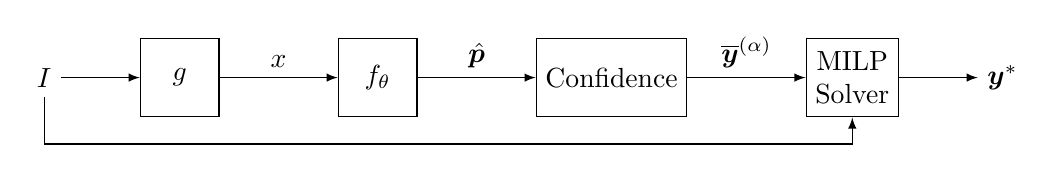
\begin{tikzpicture}
	\node (I) {$I$};
	\begin{scope}[every node/.style={draw}, align = center, minimum height = 1cm, minimum width = 1cm]
	    \node[right = of I] (g) {$g$};
	    \node[right = 1.5cm of g] (f) {$f_{\theta}$};
	    \node[right = 1.5cm of f] (conf) {Confidence};
	    \node[right = 1.5cm of conf] (solver) {MILP\\Solver};
	\end{scope}
	\node[right = of solver] (opt) {$\bm{y}^*$};

	\path [-latex] (I) edge (g);
	\path [-latex] (g) edge node [above] {$x$} (f);
	\path [-latex] (f) edge node [above] {$\hat{\bm{p}}$} (conf);
	\path [-latex] (conf) edge node [above] {$\overline{\bm{y}}^{(\alpha)}$} (solver);
	\path [-latex] (solver) edge (opt);
	\draw [-latex] (I.south) -- ++(0,-0.6cm) -| (solver.south);

    \end{tikzpicture}
    \caption{Warm-starting an MILP solver with the output of a solution prediction deep learning model. In the diagram,  $I$ is an instance of an MILP problem for which the model was trained. $g$ is an adequate embedding function. The ``Confidence'' block indicates the construction of a partial solution as described in Equation \eqref{eq:partial-solution}.}
    \label{fig:warm-starting-diagram}
\end{figure}

Note that warm-starting an MILP solver by itself does not configure a heuristic solution, as the optimality guarantees are maintained.
More precisely, warm starting a solver will only (potentially) change the order in which the nodes of the branch-and-bound tree are explored, e.g., by influencing branching decisions.
Because of that, it also maintains the optimality (and feasibility) guarantees of the MILP solver used, even if the solution prediction model provides an infeasible (partial) solution.
However, under limited time, those guarantees are lost, as the solver may be interrupted before finding even a feasible solution.
In fact, even without the warm-starting approach, the simplest matheuristic is to interrupt an MILP solver after a fixed amount of time.


\subsection{Early-fixing Variable Assignments}

Beyond merely indicating to the solver the partial solution that the deep learning model provides, it is possible to constrain the problem with that partial solution.
This early-fixing approach, also called neural diving by \citeonline{nairSolvingMixedInteger2021}, can be interpreted, given an instance $I\in \mathcal{I}$ and a partial solution as in Equation~\eqref{eq:partial-solution}, as the addition of constraints
\begin{equation}\label{eq:early-fixing-constraints}
    y_{j} = \hat{y}_j,\,\forall (j,\hat{y}_j) \in \overline{\bm{y}}^{(\alpha)}
\end{equation}
to the optimization problem.
Because such constraints limit those variables to assuming a single value, which is effectively the same as removing them from the poll of decision variables and treating them as parameters of the problem, the branch-and-bound tree gets significantly pruned.
The diagram of Figure~\ref{fig:early-fixing-diagram} illustrates this process.

\begin{figure}[h]
    \centering
    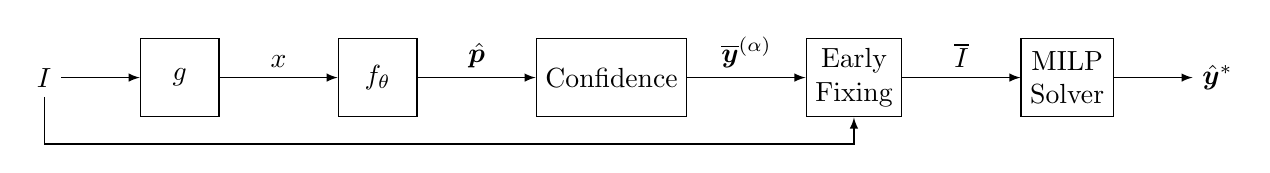
\begin{tikzpicture}
	\node (I) {$I$};
	\begin{scope}[every node/.style={draw}, align = center, minimum height = 1cm, minimum width = 1cm]
	    \node[right = of I] (g) {$g$};
	    \node[right = 1.5cm of g] (f) {$f_{\theta}$};
	    \node[right = 1.5cm of f] (conf) {Confidence};
	    \node[right = 1.5cm of conf] (ef) {Early\\Fixing};
	    \node[right = 1.5cm of ef] (solver) {MILP\\Solver};
	\end{scope}
	\node[right = of solver] (opt) {$\hat{\bm{y}}^*$};

	\path [-latex] (I) edge (g);
	\path [-latex] (g) edge node [above] {$x$} (f);
	\path [-latex] (f) edge node [above] {$\hat{\bm{p}}$} (conf);
	\path [-latex] (conf) edge node [above] {$\overline{\bm{y}}^{(\alpha)}$} (ef);
	\path [-latex] (ef) edge node [above] {$\overline{I}$} (solver);
	\path [-latex] (solver) edge (opt);
	\draw [-latex] (I.south) -- ++(0,-0.6cm) -| (ef.south);

    \end{tikzpicture}
    \caption{Early-fixing integer variables based on the output of a solution prediction deep learning model. In the diagram,  $I$ is an instance of an MILP problem for which the model was trained. $g$ is an adequate embedding function. The ``Confidence'' block indicates the construction of a partial solution as described in Equation \eqref{eq:partial-solution}. The ``Early Fixing'' block indicates the addition of constraints \eqref{eq:early-fixing-constraints}, resulting in the early-fixed instance $\overline{I}$. The solver output is written $\hat{\bm{y}}^*$ to indicate it as being a heuristic solution.}
    \label{fig:early-fixing-diagram}
\end{figure}

Naturally, the addition of the early-fixed constraints implies that there are no guarantees that the solution found is optimal.
In fact, the resulting problem instance (denoted $\overline{I}$, as in Figure~\ref{fig:early-fixing-diagram}) might be infeasible, if the added constraints come from an infeasible assignment.
However, by adjusting the parameter $\alpha$, which controls the size of the partial solution, it is possible to indirectly adjust the size of the resulting branch-and-bound tree, as a smaller value of $\alpha$ implies in more variables in the partial solution, thus, more fixing constraints, which result in a smaller tree. 
In fact, $\alpha\to 0$ reduces the early-fixing matheuristic to the naïve use of the solution predicted by the deep learning model.
Furthermore, it is easy to see that, instead of a fixed threshold $\alpha$, one can build partial solutions by picking the $n-n'$ ($n' < n$) variables that the model is most confident of, such that the resulting problem instance always has $n'$ variables and, thus, can be solved in a tractable manner.


\subsection{Trust-region}

Instead of strictly fixing the variables based on the model's output, \citeonline{hanGNNGuidedPredictandSearchFramework2023} have proposed to allow a small deviation from that value.
In other words, the solution prediction model's output is used to define a \emph{trust region} in which an MILP solver can search for the optimal solution.
Instead of constraints like in Equation~\eqref{eq:early-fixing-constraints}, the instance is modified with the addition of constraints of the form
\begin{equation}\label{eq:trust-region-constraint}
    \sum_{(j,\hat{y}_j) \in \overline{\bm{y}}^{(\alpha)}} |y_{j} - \hat{y}_j| \le \Delta
,\end{equation}
where $\Delta \in \R_+$ defines the size of the trust region.
Note how the above equation limits the space of feasible solutions to a neighborhood of the partial solution derived from the model's output.
The diagram in Figure~\ref{fig:trust-region-diagram} illustrates the trust region heuristic approach.

\begin{figure}[h]
    \centering
    \begin{tikzpicture}
	\node (I) {$I$};
	\begin{scope}[every node/.style={draw}, align = center, minimum height = 1cm, minimum width = 1cm]
	    \node[right = of I] (g) {$g$};
	    \node[right = 1.5cm of g] (f) {$f_{\theta}$};
	    \node[right = 1.5cm of f] (conf) {Confidence};
	    \node[right = 1.5cm of conf] (tr) {Trust\\Region};
	    \node[right = 1.5cm of tr] (solver) {MILP\\Solver};
	\end{scope}
	\node[right = of solver] (opt) {$\hat{\bm{y}}^*$};

	\path [-latex] (I) edge (g);
	\path [-latex] (g) edge node [above] {$x$} (f);
	\path [-latex] (f) edge node [above] {$\hat{\bm{p}}$} (conf);
	\path [-latex] (conf) edge node [above] {$\overline{\bm{y}}^{(\alpha)}$} (tr);
	\path [-latex] (tr) edge node [above] {$\overline{I}^{(\Delta)}$} (solver);
	\path [-latex] (solver) edge (opt);
	\draw [-latex] (I.south) -- ++(0,-0.6cm) -| (ef.south);

    \end{tikzpicture}
    \caption{Solving an instance of an MILP problem within a trust region based on the output of a solution prediction deep learning model. In the diagram,  $I$ is an instance of an MILP problem for which the model was trained. $g$ is an adequate embedding function. The ``Confidence'' block indicates the construction of a partial solution as described in Equation \eqref{eq:partial-solution}. The ``Trust Region'' block indicates the addition of the constraint \eqref{eq:trust-region-constraint}, resulting in the instance $\overline{I}^{(\Delta)}$ with limited solution space. The solver output is written $\hat{\bm{y}}^*$ to indicate it as being a heuristic solution.}
    \label{fig:trust-region-diagram}
\end{figure}

It is easy to see that picking $\Delta=0$ results in the early-fixing approach.
A distinguishing feature of the trust region approach is that the parameter $\Delta$ can be adjusted to turn an infeasible instance into a feasible one, or, perhaps, to include a better solution in the feasible region.
However, no optimality nor feasibility guarantees can be provided by this approach.


	
% The \phantomsection command is needed to create a link to a place in the document that is not a
% figure, equation, table, section, subsection, chapter, etc.
% https://tex.stackexchange.com/questions/44088/when-do-i-need-to-invoke-phantomsection
\phantomsection

\chapter{Offline Nanosatellite Task Scheduling}\label{chap:onts}

This chapter delves on the application area of the experiments conducted for this dissertation, specifically focusing on the Offline Nanosatellite Task Scheduling (ONTS) problem.
Over the past decade, nanosatellites have gained significant attention from both industry and academia, primarily due to their cost-effective development and launch processes~\cite{shiromaCubeSatsBrightFuture2011,luciaComputationalNanosatelliteConstellations2021,nagelNanosatellitesAppliedOptical2020,saeedCubeSatCommunicationsRecent2020}.
Despite these advantages, the limited computational and energy resources of nanosatellites present substantial challenges in mission planning.
Effective task scheduling is essential to optimize resource utilization, enhance data quality, and ensure mission success, thereby securing a return on investment.

The ONTS problem is critical for the efficient development, deployment, and operation of nanosatellites.
From launch to disposal, the ONTS problem must be solved repeatedly.
At every communication window, new schedules must be generated and deployed, and the optimal schedule is determined by an iterative procedure, exploring different sets of tasks to be performed in the schedule's timespan.
Given a nanosatellite and a collection of tasks, determining the schedule with maximum QoS is a combinatorial problem.
Mathematical formulations have been proposed for this problem, from Integer Programming (IP)~\cite{rigoTaskSchedulingOptimal2021} to Mixed Integer Linear Programming (MILP)~\cite{rigoNanosatelliteTaskScheduling2021,semanEnergyAwareTaskScheduling2022} and Continuous-Time techniques~\cite{camponogaraContinuoustimeFormulationOptimal2022}.
However, the NP-hard nature of the problem renders multiple executions of the optimization algorithms (e.g., for different task configurations) within the timespan of a communication window an efficiency challenge.

The following section will present the problem statement with a description of the factors that are taken into consideration.
Then, the MILP formulation of the problem, proposed by \citeonline{rigoNanosatelliteTaskScheduling2021}, is presented, which will be the base for the experiments presented in Part~\ref{experiments-and-results}.

% The instances to be solved share common features.
% Beyond the problem structure, which remains unaltered, tasks, orbit information, and battery capacity can be understood as being randomly drawn from an unknown distribution at every communication window.
% This setup fits the context of primal heuristics based on 
% 
% It involves determining an optimal schedule for task execution that maximizes Quality-of-Service (QoS).
% This requires careful consideration of various factors, including task priority, minimum and maximum activation events, execution time frames, periods, and execution windows.
% Additionally, the constraints imposed by the satellite's power resources and the complexities of energy harvesting and management systems must be addressed.
% By solving the ONTS problem, we can significantly improve the operational efficiency and effectiveness of nanosatellite missions, ensuring their success and sustainability.


\section{Problem Statement}

Nanosatellite scheduling problems involve making decisions regarding the start and finish times of each task.
These tasks often require periodic execution and must be scheduled during specific moments along the satellite's orbit.
In addition to temporal constraints, energy availability throughout the orbit is a crucial resource that must be taken into account.
Figure \ref{fig:example-scheduling} illustrates an example of optimal scheduling, where each job is represented by a different color, and the activation and deactivation of tasks are depicted as steps in the signal sequence.

\begin{figure}[h]
    \centering
    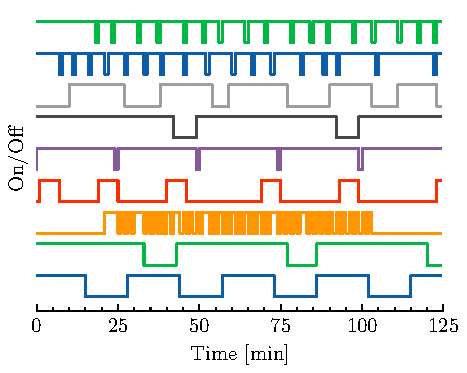
\includegraphics{schedule_example.pdf}
    \caption{Illustration of an optimum scheduling for 9 tasks on a horizon of 125 time steps. Each color represents the executions of a different task.}
    \label{fig:example-scheduling}
\end{figure}

Effective scheduling must incorporate energy management to ensure that tasks do not consume more energy than the system can provide, thereby preventing the battery from depleting before the mission concludes.
Energy management is particularly challenging because the nanosatellite relies on solar panels for power.
The energy availability is influenced by the nanosatellite's attitude, which affects the orientation of the solar panels, and its trajectory relative to Earth's shadow, as depicted in Figure \ref{fig:onts-orbit}.
On top of that, the shared energy resources steps up the problem complexity, as each task's activation must be determined while taking into consideration the other tasks.

\begin{figure}[h]
    \centering
    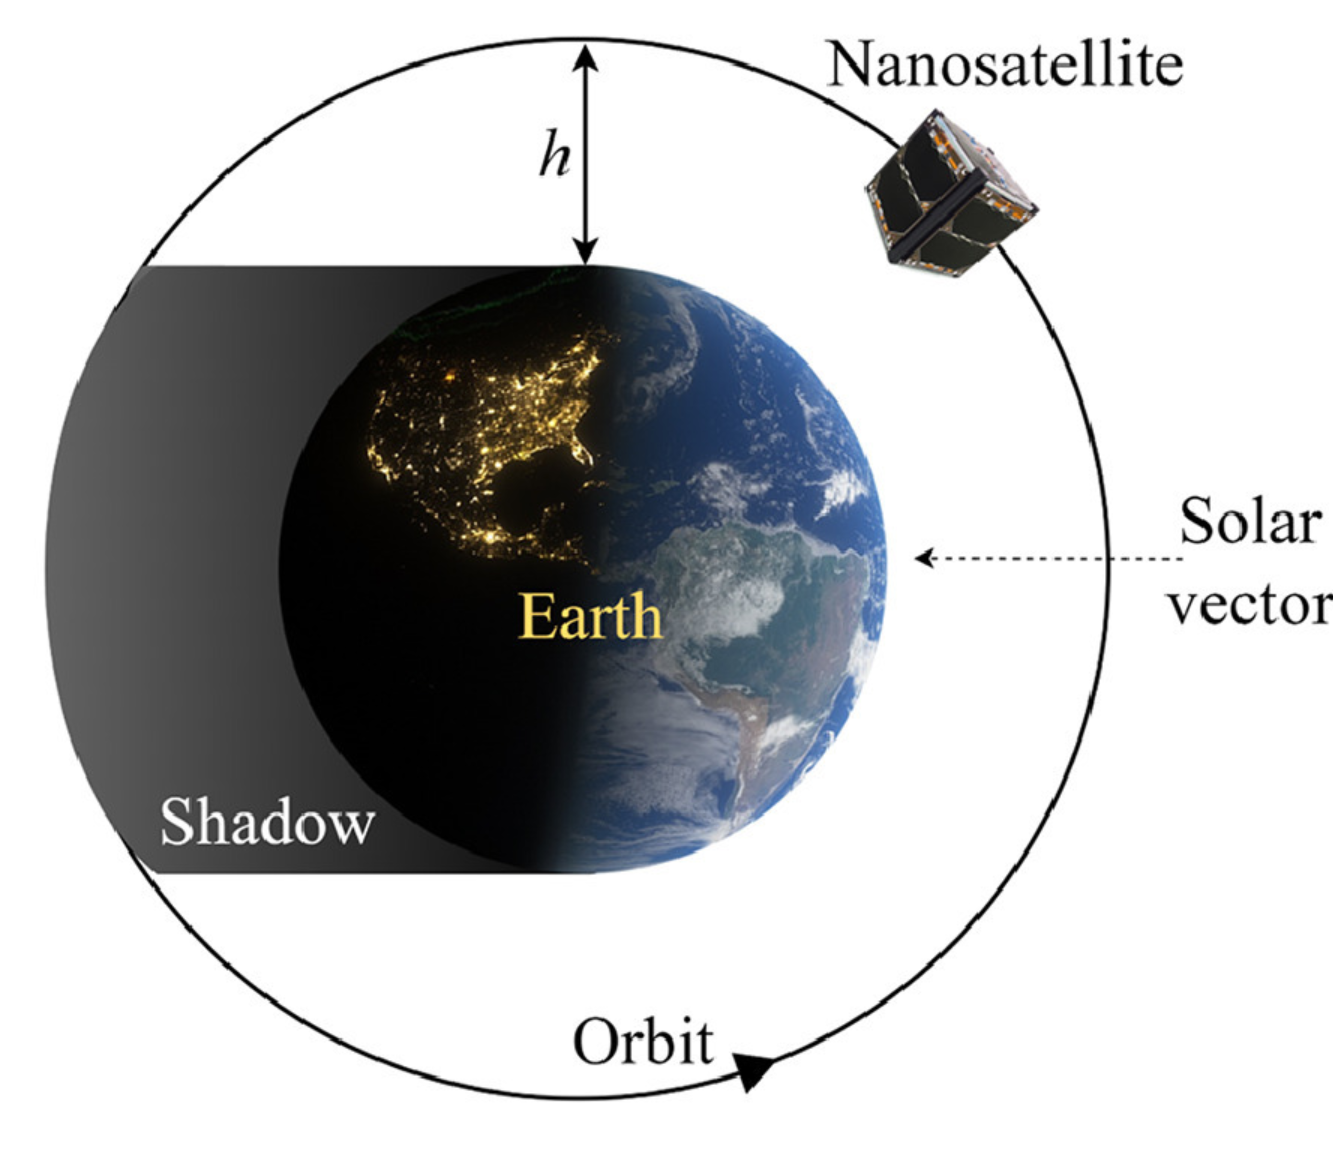
\includegraphics[width=0.5\textwidth]{onts_orbit.png}
    \caption{Illustration of a nanosatellite's orbit around Earth. Image from \citeonline{rigoBranchandpriceAlgorithmNanosatellite2022}.}
    \label{fig:onts-orbit}
\end{figure}


\section{MILP Problem}

The formulation presented here was proposed by \citeonline{rigoTaskSchedulingOptimal2021} and the reader is advised to refer to the original work for further details.

Given a set $\mathcal{J}=\{1,...,J\}$ of tasks (or jobs), and a set $\mathcal{T}=\{1,...,T\}$ of time units of the scheduling horizon, let variables $x_{j,t}$ represent the allocation of task $j$ at time $t$, $\forall j\in \mathcal{J}, \forall t\in \mathcal{T}$.
Naturally, each $x_{j,t}$ is a binary variables, in which value $1$ indicates that task $j$ is scheduled to be in execution at time $t$.
When convenient, these variables will be represented as a vector \[
    % \bm{x}=(x_{1,1},\ldots,x_{1,T},\ldots,x_{J,1},\ldots,x_{J,T})
    \bm{x} = \left( x_{j,t} \right)_{\substack{j=1,\ldots,J\\ t=1,\ldots,T}}
,\] which is a notation also used for other variables and parameters.

Every task $j$ has an associated priority $u_j > 0$, such that the mission's QoS is defined as
\begin{equation}\label{eq:qos}
    {\rm QoS}(\bm{x};\bm{u}) = \sum_{j=1}^{J} \sum_{t=1}^{T} {u}_{j} x_{j,t}
.\end{equation}
As mentioned previously, the goal of the optimization problem is to find a schedule that maximizes the QoS.

Auxiliary variables $\phi_{j,t}$ are defined for every $j\in \mathcal{J}$ and $t\in \mathcal{T}$, which represent the startup of the task, i.e, $\phi_{j,t} = 1$ indicates that task $j$ is not running at time $t-1$ but its execution is started at time $t$.
The behavior of these auxiliary variables is ensured by
\begin{equation}\label{eq:phi-constraints}
    \begin{aligned}
	& \phi_{j,t} \geq x_{j,t}, &~\forall j\in\mathcal{J},\, t = 1  \\
        & \phi_{j,t} \geq x_{j,t} - x_{j,(t-1)}, &~\forall j\in\mathcal{J}, \,\forall t\in\mathcal{T}: t > 1   \\
        & \phi_{j,t} \leq x_{j,t}, &~\forall j\in\mathcal{J}, \,\forall t\in\mathcal{T}   \\
        & \phi_{j,t} \leq 2 - x_{j,t} - x_{j,(t-1)}, &~\forall j\in\mathcal{J}, \,\forall t\in\mathcal{T}: t > 1
    .\end{aligned}
\end{equation}

The multiple requirements of each task are ensured by a series of constraints.
Each task $j$ may run only during a specified time window delimited by $w_{j}^{\text{min}}$ and $w_{j}^{\text{max}}$, which is imposed by
\begin{equation}\label{eq:window-constraints}
    \begin{aligned}
        &\sum_{t=1}^{\textcolor{black}{w^{\min}_{j}}} x_{j,t} = 0,  & \forall j\in\mathcal{J} \\
        &\sum_{t=w^{\max}_{j}+1}^{T} x_{j,t} = 0, & \forall j\in\mathcal{J}
    .\end{aligned}
\end{equation}
Such constraints can be used to force a task to be executed when the nanosatellite is passing over a predetermined region.

To limit continuous executions, a task $j$ is constrained to stop for at least $t_j^{\text{min}}$, and at most $t_j^{\text{max}}$ time steps by
\begin{equation}\label{eq:execution-gap-constraints}
    \begin{aligned}
        &\sum_{l=t}^{t+{t}^{\min}_{j}-1} x_{j,l} \geq {t}^{\min}_{j} \phi_{j,t},  &\forall t \in \{1,...,T-{t}^{\min}_{j} + 1\}, \forall j\in\mathcal{J} \\
        &\sum_{l=t}^{t+{t}^{\max}_{j}} x_{j,l} \leq {t}^{\max}_{j},  &\forall t \in \{1,...,T-{t}^{\max}_{j}\}, \forall j\in\mathcal{J}
    .\end{aligned}
\end{equation}
Complementary, and having in mind that the end of schedule is not the end of the nanosatellite life, the addition of constraint
\begin{equation}\label{eq:execution-end-constraints}
    \begin{aligned}
        &\sum_{l=t}^{T} x_{j,l} \geq (T - t + 1) \phi_{j,t},  & \forall t \in \{T-{t}^{\min}_{j} + 2,...,T\}, \forall j\in\mathcal{J}
    \end{aligned}
\end{equation}
enables the start of the execution of a task close to the end of the schedule horizon, and keep it running until the end.

For a task to be executed periodically, at least every $p_j^{\text{min}}$ time steps, and at most every $p_j^{\text{max}}$ time steps, the following constraints are added:
\begin{equation}\label{eq:prediodicity-constraints}
    \begin{aligned}
        &\sum_{l=t}^{t+{p}^{\min}_{j}-1} \phi_{j,l} \leq 1,   & \forall t \in \{1,...,T-{p}^{\min}_{j}+1\}, \forall j\in\mathcal{J}  \\
        & \sum_{l=t}^{t+{p}^{\max}_{j}-1} \phi_{j,l} \geq 1,  & \forall t \in \{1,...,T-{p}^{\max}_{j}+1\},  \forall j\in\mathcal{J} 
    .\end{aligned}
\end{equation}
On top of that, a task may be required to run multiple times over the planning horizon.
The constraints
\begin{equation}\label{eq:multiple-execs-constraints}
    \begin{aligned}
        &\sum_{t=1}^{T} \phi_{j,t} \geq {y}^{\min}_{j}, &\forall j\in\mathcal{J}   \\
        &\sum_{t=1}^{T} \phi_{j,t} \leq {y}^{\max}_{j}, &\forall j\in\mathcal{J}
    \end{aligned}
\end{equation}
are added to ensure at least $y_{j}^{\text{min}}$ and at most $y_j^{\text{max}}$ runs are performed for task $j$.

The energy-management restrictions are ensured through multiple constraints.
Given $r_t$, the power available from the solar panels at each time $t$, $q_j$, the power required by each task $j$, and $\gamma~V_{b}$, the maximum power the battery can provide, then
\begin{equation}\label{eq:power-consumption-constraints}
    \begin{aligned}
	&\sum_{j=1}^{J} q_{j} x_{j,t} \leq r_t + \gamma~V_{b}, & \forall t\in\mathcal{T}
    \end{aligned}
\end{equation}
limits the power consumption to realistic levels.
Auxiliary variables $b_t$ and $\text{SoC}_t$ represent, resp., the exceeding power and the State of Charge (SoC) over each time $t\in \mathcal{T}$.
Given $Q$, the battery capacity, and $e$, the discharge efficiency, the exceeding power is ensured by
\begin{equation}\label{eq:exceeding-power-constraints}
    \begin{aligned}
	& b_{t} = r_{t} - \sum_{j \in \mathcal{J}} q_{j} x_{j,t}, &  \forall t \in \mathcal{T}
    ,\end{aligned}
\end{equation}
while the SoC is ensured by
\begin{equation}\label{eq:SoC-constraints}
    \begin{aligned}
    &\text{SoC}_{t+1} = \text{SoC}_{t} + \frac{b_{t}~e}{60~Q~V_{b}}, & \forall t \in \mathcal{T}  \\
    &\text{SoC}_{t} \leq 1, & \forall t\in\mathcal{T}    \\
    &\text{SoC}_{t} \geq \rho, & \forall t\in\mathcal{T}
    ,\end{aligned}
\end{equation}
where $\rho$ is the allowed lower limit for the battery, which is usually greater than zero for safety purposes.

Finally, the ONTS problem is formulated as an MILP
\begin{equation}\label{eq:onts-milp}
\begin{aligned}
    \max_{\bm{x},\bm{\phi},\bm{\text{SoC}},\bm{b}} \quad & \eqref{eq:qos} \\
    \textrm{s.t.} \quad & (\ref{eq:phi-constraints} \text{--} \ref{eq:SoC-constraints}) \\
	    & x_{j,t}, \phi_{j,t} \in \left\{ 0,1 \right\} ,\quad \forall j\in \mathcal{J}, t\in \mathcal{T} \\
.\end{aligned} \tag{ONTS}
\end{equation}
Note that the constraints \eqref{eq:exceeding-power-constraints} and \eqref{eq:SoC-constraints} imply that the continuous variables $\bm{b}$ and $\bm{\text{SoC}}$ are uniquely determined by a given assignment for the binary variables $\bm{x}$ and $\bm{\phi}$.
Therefore, the problem can be reduced to finding an assignment $\bm{y}=(\bm{x},\bm{\phi}) \in \left\{ 0,1 \right\}^{n}$, where $n=2JT$.

Let $\mathcal{I}$ be the space of all MILP problems of the form \eqref{onts-milp}.
Any instance $I\in \mathcal{I}$ is parameterized by $\pi_I = \left( \bm{u}, \bm{q}, \bm{y}^{\min}, \bm{y}^{\max}, \bm{t}^{\min}, \bm{t}^{\max}, \bm{p}^{\min}, \bm{p}^{\max}, \bm{w}^{\min}, \bm{w}^{\max}, \bm{r}, \rho, e, Q, \gamma, V_b \right) $, and, implicitly, by the number of tasks $J$ and the number of time units $T$.
Let $\Pi^{J,T}$ denote the space of parameter vectors as above, such that any instance $I\in \mathcal{I}$ can be uniquely determined by a parameter vector $\pi_{I}$ (given adequate $J$ and $T$).



	
% The \phantomsection command is needed to create a link to a place in the document that is not a
% figure, equation, table, section, subsection, chapter, etc.
% https://tex.stackexchange.com/questions/44088/when-do-i-need-to-invoke-phantomsection
\phantomsection

\chapter{Evaluation of Primal Heuristics}\label{chap:evaluation}

As discussed in Chapter\,\ref{chap:integer-programming}, Section\,\ref{sec:heuristics}, a primal heuristic abides from optimality guarantees to focus on a trade-off between solution quality and computational cost (speed).
Consequently, two primal heuristics for MILP problems can be compared with respect to how fast they provide solutions and how good they are, and whether the solutions are feasible or not.
% In this chapter, two approaches are discussed to evaluate primal heuristics.
In this chapter, multiple metrics are presented to cover the two perspectives in which a heuristic can be said superior to another.
% The first (Sec.~\ref{sec:standard-evaluation-metrics}) is based on standard evaluation metrics. Therefore, it uses multiple metrics, one for each
% The second (Sec.\,\ref{sec:primal-integral}) is specific to primal heuristics that improve the candidate solution over time, such as matheuristics.
% By tracing the progress of the candidate solution, it provides a single metric that takes into account the characteristic trade-off of primal heuristics.

% - como discutido na sec XXX, ao abrir mão da garantia de otimalidade, uma heurística primal oferece a possibilidade de trocar qualidade da solução por velocidade de otimização.
% - nesse sentido, duas heurísticas podem ser comparadas em função dessa relação
% - neste capítulo, duas abordagens serão apresentadas para caracterizar a qualidade de heurísticas. a primeira, através de múltiplas métricas que são comumente para avaliar qualquer tipo de heurística
% - a segunda, específica para matheuristics, que explora a sua característica de aprimorar a solução candidata ao longo do tempo

% \phantomsection
\section*{}
% \section{Standard Evaluation Metrics}\label{sec:standard-evaluation-metrics}

The objective value and the time taken to provide a solution are natural evaluation metrics.
However, they have significant shortcomings.
The value of the cost function (supposing a minimization problem) is hard to interpret without bounds.
For example, it is difficult to judge how better one heuristic approach is with respect to the other just by knowing that the first provided a solution with a cost of 10, while the second provided a solution with a cost of 15.
If the optimal solution costs -1000 and a trivial solution costs 20, then it can be said that both heuristics performed poorly.
On the other hand, if the optimal solution has a cost of 9 and a trivial solution has cost 15, then it can be said that the first heuristic performed much better than the second.

Therefore, to make a fair judgment about the solution quality of a set of heuristics being evaluated, one needs to know both the cost of the solutions as well as upper and lower bounds for the problem.
Beyond the difficulty of determining such bounds, having a multidimensional metric for judging solution quality can make it more challenging to compare the performance across different optimization problems and even across different instances of the same problem.
An alternative to summarizing all these values is to compute the cost of the heuristic solution normalized between the optimal cost (0~\%) and the cost of the trivial solution (100~\%).
Let $\hat{\bm{y}}$ be a heuristic solution, $\bm{y}^*$ be the optimal solution, and $\overline{\bm{y}}$ be a trivial solution for an instance of an optimization problem as in \eqref{eq:general-milp}.
Then, \emph{relative cost} of $\hat{\bm{y}}$ can be defined as
\begin{equation}
    \text{RelCost}(\hat{\bm{y}}) = \frac{\bm{c}^{T} \hat{\bm{y}} - \bm{c}^{T} \bm{y}^*}{\bm{c}^{T}\overline{\bm{y}} - \bm{c}^{T}\bm{y}^*}
.\end{equation}

Similarly, if the problem of interest is a maximization problem, then one can define the \emph{relative objective} of a candidate solution $\hat{\bm{y}}$ as
\begin{equation}\label{eq:relobj}
    \text{RelObj}(\hat{\bm{y}}) = \frac{\bm{c}^{T} \hat{\bm{y}}  - \bm{c}^{T}\overline{\bm{y}}}{\bm{c}^{T}\bm{y}^* - \bm{c}^{T}\overline{\bm{y}}}
.\end{equation}

Certain conditions must be met to evaluate an approach's efficiency, ensuring that the time taken to compute a solution (runtime) is meaningful and fair.
One way to do so is to ensure that the computational resources are fairly available to all approaches.
Usually, this implies in allowing all approaches to have plain access to a common hardware, i.e., that there are no other processes using the resources during the time of execution.

Still, there are a few caveats in this performance metric, of which parallelization abilities are probably the most prominent.
Comparing single-process with multi-process approaches is quite difficult, as a process that can compute its results in parallel uses more resources in the same runtime. 
Furthermore, projecting empirical results to different setups is challenging when the processes being evaluated use parallel computation. 
% An alternative would be to compute the total computational time, e.g., if a process is running 
In this work, it is considered that parallelization is commonly supported in modern hardware configurations.
Thus, the runtime is computed as the user-perceived real time (or wall time) for the heuristic to provide a solution given an instance of an optimization problem, regardless of whether parallelization was used or not.

% \section{The Primal integral}\label{sec:primal-integral}

% % see https://www.ecole.ai/2021/ml4co-competition/#metrics

% Although relative cost can be used to compare heuristics given a fixed time budget, it does not properly suit the cases where the time taken by a heuristic has a variable cost.
% For such cases, it is possible to use the integral of the relative cost over time, or the \emph{primal integral}, as used in \citeonline{gasseMachineLearningCombinatorial2022}.
% To see this, consider a heuristic that provides increasingly better solutions over time.
% One could define the cost at time $t$ as the cost associated with the best solution up to time $t$.
% Figure~\ref{fig:primal-curve} illustrates the evolution of the cost over time (orange curve).
% The primal integral is precisely the integral of such cost over time, which can be written \[
%     \int \bm{c}^T \hat{\bm{y}}(t) dt
% ,\] where $\hat{\bm{y}}(t)$ is the best solution known (or candidate solution) at time $t$.
% It is called the primal integral because it computes the integral of the cost associated with primal solutions.

% \begin{figure}[h]
%     \centering
%     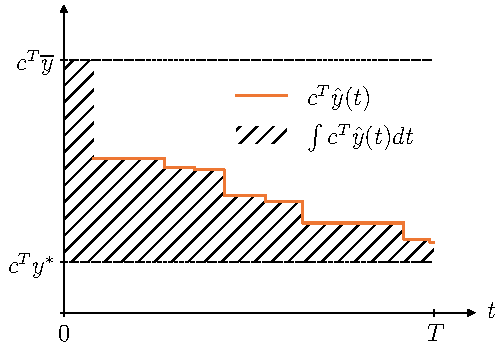
\includegraphics{primal.pdf}
%     \caption{Example of primal integral computation. $y^*$ and $\overline{y}$ are (sub-)optimal and trivial solutions, respectively. The orange curve represents the evolution of the candidate solution's cost over time. Note that the orange curve is not defined at the beginning of the runtime, indicating that a candidate solution is not provided at $t=0$. The hatched area is the primal integral, bounded by the two references ($y^*$ and $\overline{y}$).}
%     \label{fig:primal-curve}
% \end{figure}

% The straightforward integral of the primal curve, however, has two major limitations.
% First, it is not properly defined at $t \to 0$, as it is not expected that a heuristic starts with a candidate solution, i.e., $\hat{y}(0)$ is not defined.
% Furthermore, the length of this undefined region varies from heuristic to heuristic, which hinders fair comparisons.
% One way to circumvent this problem is to assume that $\hat{\bm{y}}(t) = \infty$ before the first candidate solution is provided, and compute the integral of the minimum between $\bm{c}^T \hat{\bm{y}}$ and $\bm{c}^T\overline{\bm{y}}$ (the cost of a trivial solution).
% This way, a heuristic approach is penalized for taking longer to provide a candidate solution.

% The second limitation is that the result is not comparable across different instances of a problem.
% This is because the cost of a candidate solution is meaningless, unless it is necessary to understand how close to the optimal and how far from trivial that given solution is.
% One way to attenuate this problem is to normalize the integral with respect to the difference between the cost of the trivial solution and the cost of the optimal solution.
% This approach can be interpreted as normalizing the integrals with respect to the integral of the naïve heuristic, which is simply to guess the trivial solution.

% In summary, the practical primal integral of a heuristic $H$ that can provide candidate solutions over time $\hat{\bm{y}}_H(t)$ is defined as
% \begin{equation}\label{eq:primal-integral}
%     \text{PrimalIntegral}(H) = \frac{1}{T(\bm{c}^T \overline{\bm{y}} - \bm{c}^T \bm{y}^*)} \int_0^{T} \left( \min\left( \bm{c}^T \overline{\bm{y}}, \bm{c}^{T} \hat{\bm{y}}_H(t) \right)  - \bm{c}^{T} \bm{y}^* \right)  dt
% ,\end{equation}
% where $\overline{\bm{y}}$ is a trivial solution and $\bm{y}^*$ is an optimal solution.
% Such is illustrated in Fig.~\ref{fig:primal-curve} through the hatched region.



	\part{Experiments and Results}\label{experiments-and-results}

	
% The \phantomsection command is needed to create a link to a place in the document that is not a
% figure, equation, table, section, subsection, chapter, etc.
% https://tex.stackexchange.com/questions/44088/when-do-i-need-to-invoke-phantomsection
\phantomsection

\chapter{Experiments}\label{chap:experiments}

To address the objective of this dissertation, experiments are conducted to evaluate learning-based primal heuristics for Mixed-Integer Linear Programming (MILP).
The ONTS problem (see Chap.~\ref{chap:onts}) serves as a realistic application to benchmark the selected techniques.

As discussed in Section~\ref{sec:onts-problem-statement}, during mission execution (with the nanosatellite in orbit), a new schedule must be generated during the communication window.
This involves optimizing multiple instances of the ONTS problem, given varying sets of tasks and updated nanosatellite information.
Each set of tasks is evaluated based on the resulting schedule, in an iterative process of including new tasks until scheduling becomes infeasible.
Therefore, during the communication window, quickly finding a good solution to a problem instance is more crucial than finding an optimal solution.
In other words, an efficient heuristic is crucial to allow for more iterations, which leads to a better set of tasks scheduled for execution.

The remaining of this chapter details the development and the experiments with the proposed learning-based heuristics for the ONTS problem.
This includes data acquisition, solution prediction model architecture, model training, and experiment setup.
Furthermore, the performance of the proposed learning-based heuristics is assessed on realistic instances of the ONTS problem.


\section{Data}

High-quality data is necessary both to train solution prediction models and to evaluate the proposed learning-based heuristics for the ONTS problem.
The datasets for both training and evaluation must be composed of instance-solution pairs, as discussed in Sec.~\ref{sec:training-solution-prediction}.
The quality of these instance-solution pairs is measured through their faithfulness, both the instance with respect to the true data distribution, and the solution with respect to the optimal.

\subsection{Instance space: the FloripaSat I mission}

The instance space is defined from the parameters of the FloripaSat-I mission~\cite{marcelinoCriticalEmbeddedSystem2020}.
Their nanosatellite is in orbit at an altitude of 628 kilometers and an orbital period of 97.2 minutes.
The planning horizon is fixed at $T=125$ time slots, with one slot per minute, to account for a continuous scheduling, allowing for task executions that extend the communication window.
Any instance $I\in \mathcal{I}$ has either 9, 13, 18, 20, 22, or 24 tasks.

Once the orbit of the FloripaSat-I is stable and its received solar flux is constant, the power input vector $\bm{r}$ can be calculated deterministically from solar irradiance measurements as in \citeonline{morschfilhoComprehensiveAttitudeFormulation2020}.
2 years of solar irradiance data is used as a basis for the power input vectors of the instances in the instance space.
The set $R$ is used to denote all possible values of $\bm{r}$ from the historical data.
The other battery-related parameters (see Sec.~\ref{sec:onts-milp-formulation}) are fixed as 
\begin{align*}
    e &= 0.9 \\
    Q &= 5 \\
    \gamma &= 5 \\
    V_b &= 3.6 \\
    \rho &= 0.0
\end{align*}

The remaining parameters are constrained to ranges that match previous works in the area~\cite{rigoBranchandpriceAlgorithmNanosatellite2022,semanEnergyAwareTaskScheduling2022,rigoTaskSchedulingOptimal2021}.
Therefore, following the notation established in Sec.~\ref{sec:onts-milp-formulation}, the parameter space is defined as \[
\Pi = \bigcup_{\substack{J \in \left\{ 9,13,18,20,22,24 \right\} \\ T \in \left\{ 125 \right\} }} \Pi^{J,T}
,\] where each $\Pi^{J,T}$ is such that a parameter vector \[
\pi_I= \left( \bm{u}, \bm{q}, \bm{y}^{\min}, \bm{y}^{\max}, \bm{t}^{\min}, \bm{t}^{\max}, \bm{p}^{\min}, \bm{p}^{\max}, \bm{w}^{\min}, \bm{w}^{\max}, \bm{r}, \rho, e, Q, \gamma, V_b \right)
\] belongs to $\Pi^{J,T}$ if, and only if,
\begin{equation*}
\begin{aligned}
&\begin{rcases}
    & u_j \in [1, J] \\
	 & q_j \in [0.3, 2.5] \\
    	 & y_j^{\min} \in [1, \lceil T/45 \rceil] \\
    	 & y_j^{\max} \in [y_j^{\min}, \lceil T/15 \rceil] \\
    	 & t_j^{\min} \in [1, \lceil T/10 \rceil] \\
    	 & t_j^{\max} \in [t_j^{\min}, \lceil T/4 \rceil] \\
    	 & p_j^{\min} \in [t_j^{\min}, \lceil T/4 \rceil] \\
    	 & p_j^{\max} \in [p_j^{\min}, T] \\
    	 & w_j^{\min} \in [0, \lceil T/5 \rceil] \\
    	 & w_j^{\max} \in [\lfloor T-\lceil T/5 \rceil \rfloor, T]
\end{rcases} \forall j =1,\ldots,J \\
    &\quad \bm{r} \in R \\
    &\quad e = 0.9 \\
    &\quad Q = 5 \\
    &\quad \gamma = 5 \\
    &\quad V_b = 3.6 \\
    &\quad \rho = 0.0
.\end{aligned}
\end{equation*}
Finally, the input space is then define from the parameter space, such that \[
    I\in \mathcal{I} \iff \pi_I \in \Pi 
.\] 


\subsection{Data acquisition}

As historical data is not available for the ONTS problem, the dataset is built from randomly generated instances sampled uniformly from the instance space of the FloripaSat-I mission.
More precisely, the dataset is built with instances drawn uniformly from the instance space defined above.

As the addition of an element to the dataset requires a solution to the ONTS problem, the computational cost of building a large dataset with hard instances is very high.
To alleviate this cost, the training set is built solely with instances with fewer tasks, which are, on average, faster to solve than instances with many tasks.
However, the instances of interest are those with plenty of tasks, which are harder to solve in practice, and, thus, motivate the use of heuristics.
Therefore, the validation and test datasets are built from instances with many tasks, which are, on average, significantly harder to solve.
Table~\ref{tab:dataset} details the number of instances by size (number of tasks) in each dataset generated.

\begin{table}[h]
    \centering
    \caption{Number of instances by size in each dataset. The datasets were generated through Algorithm~\ref{alg:dataset-generation}.}
    \label{tab:dataset}
    \begin{tabular}{l | c | c | c}
    \toprule
    & Training & Validation & Test \\
    \midrule
    $J = 9$ & 200 & 0 & 0 \\
    $J = 13$ & 200 & 0 & 0 \\
    $J = 18$ & 200 & 0 & 0 \\
    $J = 20$ & 0 & 20 & 20 \\
    $J = 22$ & 0 & 20 & 20 \\
    $J = 24$ & 0 & 20 & 20 \\
    \midrule
    Total & 600 & 60 & 60 \\
    \bottomrule
    \end{tabular}
\end{table}

Distinguishing the size of the instances in each dataset allows for the construction of a large training set, which enables the models to properly learn the problem, while maintaining a challenging evaluation scenario.
On top of that, this approach also enables the evaluation of the generalization capabilities of the proposed solution prediction models and the derived learning-based heuristics.

The algorithm to generate the datasets is presented in Algorithm~\ref{alg:dataset-generation}.
As the time horizon is fixed, the algorithm is executed once for each number of tasks possible.
Every new instance $I$ is solved using the SCIP solver~\cite{bestuzhevaSCIPOptimizationSuite2021} with a limited time budget of 5 minutes.
An instance is rejected if no feasible solution is found during the time budget or if the solver proves infeasibility.
For each instance $I$ in the resulting dataset, the set $Z^*_I$ contains the best 500 solutions found by the solver.

\begin{algorithm}[h]
    \NoCaptionOfAlgo
    \SetAlgoLined
    \KwData{Time horizon $T$, number of jobs $J$, number of instances (final dataset size) $n$.}
    \KwResult{Dataset $\mathcal{D} = \{(I,Z_I^\star): Z_I^\star\subset Z_I\}$.}
    
    \While{$|\mathcal{D}| < n$}{
        $\pi \sim \mathcal{U}\left( \Pi^{J,T} \right) $ \\
        $I \gets {\tt ONTS}(\pi)$ \\
        $Z_I^\star \gets {\tt Solver}(I)$
        
        \If{$|Z_I^\star| > 0$}{%
            $\mathcal{D}$.add$(I, Z_I^\star)$
        }
    }
    \caption{\textbf{Algorithm 1:} Dataset generation algorithm. $\pi$ is the parameter vector and $\Pi^{J,T}$ is the parameter space (see Sec. \ref{sec:onts-milp-formulation}), $Z_I$ represents the set of all feasible solutions of instance $I$, and $Z_I^\star \subset Z_I$ the set of feasible solutions the solver finds.
    ${\tt ONTS}$ represents a function that takes as input a parameter vector and constructs an instance of the ONTS problem.
    ${\tt Solver}$ is any MILP solver.
    Note that the parameters are drawn uniformly from the parameter space.
    }\label{alg:dataset-generation}
\end{algorithm}


\section{Deep Learning Model Architectures}

- GNNs are very promising, considered sota
- FCNs are not suitable for our problem, because it must suit instances with varying number of jobs (and, thus, varying number of variables), while FCNs have a fixed output dimension.

\section{Training}

\section{Evaluation}



	% \phantompart

	% \phantomsection
% 
% % https://tex.stackexchange.com/questions/5076/is-it-possible-to-keep-my-translation-together-with-original-text
% \chapter*{Conclusion}\label{chap:conclusion}
% \addcontentsline{toc}{chapter}{Conclusion}
% \phantomsection

\chapter*{Conclusion}\label{conclusion}
\addcontentsline{toc}{part}{Conclusion}
\markboth{Conclusion}{Conclusion}


This dissertation evaluates the effectiveness of primal heuristics for Mixed-Integer Linear Programming (MILP) that leverage deep learning-based solution prediction models.
The overarching goal was to contribute towards answering the three foundational questions posed in the \nameref{chap:intro} regarding the design, training, and integration of these models in primal heuristics.

The key contributions of this work were presented in Chapters~\ref{chap:solution-prediction}, \ref{chap:experiments}, and \ref{chap:discussion}.
The Offline Nanosatellite Task Scheduling (ONTS) problem served as the application context, providing a challenging benchmark for evaluating the techniques of interest.

First, the architectural components of solution prediction models were analyzed.
The selected architecture was based on graph neural networks (GNNs) with layers featuring two half-convolutions, a structure commonly employed in similar optimization problems~\cite{gasseExactCombinatorialOptimization2019,nairSolvingMixedInteger2021,khalilMIPGNNDataDrivenFramework2022,cappartCombinatorialOptimizationReasoning2022}.
Experiments demonstrated that the SAGE operator~\cite{hamiltonInductiveRepresentationLearning2017} outperformed the original operator proposed by \citeonline{kipfSemiSupervisedClassificationGraph2017}.
Additionally, the approach of sharing parameters between the two half-convolutions yielded the best-performing models.

Two distinct approaches for training solution prediction models were implemented and evaluated.
The results indicated that using multiple solutions from a given instance as targets during training, as suggested by \citeonline{nairSolvingMixedInteger2021}, produced more confident and effective models compared to using only a (quasi-)optimal solution.

Another aspect of training solution prediction models evaluated during the experiments is data acquisition.
In the absence of enough historical data, a common challenge to be overcome is the high cost of generating enough data for training solution prediction models~\cite{bengioMachineLearningCombinatorial2021,cappartCombinatorialOptimizationReasoning2022,pmlr-v119-yehuda20a}.

Data acquisition emerged as a significant challenge, particularly in the absence of sufficient historical data, due to its high computational cost~\cite{bengioMachineLearningCombinatorial2021,cappartCombinatorialOptimizationReasoning2022,pmlr-v119-yehuda20a}.
However, the experiments demonstrated that the GNN architecture could generalize well to instances \emph{harder}\footnote{In terms of computational cost.} than those seen during training, alleviating some of the data acquisition costs.
This finding aligns with the results of \citeonline{gasseExactCombinatorialOptimization2019}, underscoring the robustness and versatility of GNNs in this context.

Finally, the incorporation of solution prediction models into primal heuristics was investigated through experiments with three matheuristic strategies compared to a baseline MILP solver with limited time.
The approach of early-fixing integer variables based on model predictions consistently outperformed both the trust-region and warmstarting heuristics.
This strategy not only provided the best solutions within limited time frames but also found feasible solutions more rapidly.

In summary, this dissertation demonstrated that deep learning-based primal heuristics offer a promising avenue for addressing the challenges of MILP.
The research contributes to the growing field of machine learning for combinatorial optimization by providing a thorough evaluation of these heuristics' practical benefits in a representative application.
By achieving its objectives and offering valuable insights into the development and application of these heuristics, this work lays the groundwork for further advancements, ultimately contributing to more efficient and adaptable optimization solutions in practice.

Looking ahead, future research should explore the limits of the generalization capacity of GNNs in combinatorial optimization contexts.
Understanding these limits more precisely could improve estimates of the trade-off between data acquisition cost and model performance, potentially reducing the overall cost of training solution prediction models.
Additionally, enhancing instance generation techniques will be crucial for better supporting the training of deep learning models.
As highlighted by \citeonline{smith-milesGeneratingNewTest2015}, the quality of generated instances is vital for both training and evaluation.
Improved instance generation could not only lower data acquisition costs but also enhance confidence in the models' outputs, further advancing the field.

% Additionally, exploring the integration of unsupervised learning techniques can generate a significant impact by approximating the loss function to the target function to be modeled.
% The usual entropy-based loss functions do not capture the intricacies of optimal and feasible solutions, which are the \emph{de facto} targets of solution prediction models.
% Thus, unsupervised learning techniques 

% Additionally, the evaluation of other consolidated learning techniques that are of practical interest should help build the confidence in learning-based primal heuristics, approximating them from widespread application.
% Examples of such techniques are regularization, data augmentation, and online learning, which, although commonly applied in traditional deep learning tasks, have their caveats when training GNNs on optimization problems.


	
	% ----------------------------------------------------------
	% ELEMENTOS PÓS-TEXTUAIS
	% ----------------------------------------------------------
	\postextual
	% ----------------------------------------------------------
	
	% ----------------------------------------------------------
	% Referências bibliográficas
	% ----------------------------------------------------------
	\bibliographystyle{abntex2-alf}
	\bibliography{aftertext/references.bib}
	
	% ----------------------------------------------------------
	% Glossário
	% ----------------------------------------------------------
	%
	% Consulte o manual da classe abntex2 para orientações sobre o glossário.
	%
	%\glossary
	
	% ----------------------------------------------------------
	% Apêndices
	% ----------------------------------------------------------
	
	% ---
	% Inicia os apêndices
% 	% ---
 	% \begin{apendicesenv}
       	% 
 	% 	% Imprime uma página indicando o início dos apêndices
 	% 	\partapendices
 	% 	


%
% How to fix the Underfull \vbox badness has occurred while \output is active on my memoir chapter style?
% https://tex.stackexchange.com/questions/387881/how-to-fix-the-underfull-vbox-badness-has-occurred-while-output-is-active-on-m
%

% ---

\lang
{\chapter[Page not filled]{Since this page is not being completely filled, it is generating the bottom bottom of the page}}
{\chapter[Página não gerada]{Como esta página não está sendo completamente preenchida, ele está gerando a caixa inferior inferior da página}}
% ---


% Multiple-language document - babel - selectlanguage vs begin/end{otherlanguage}
% https://tex.stackexchange.com/questions/36526/multiple-language-document-babel-selectlanguage-vs-begin-endotherlanguage
\begin{otherlanguage*}{english}

\showfont

1. How to display the font size in use in the final output,
2. How to display the font size in use in the final output,
3. How to display the font size in use in the final output,
4. How to display the font size in use in the final output,
5. How to display the font size in use in the final output,
6. How to display the font size in use in the final output,
7. How to display the font size in use in the final output,
8. How to display the font size in use in the final output,
9. How to display the font size in use in the final output,


% As this page is not being completely filled, it is generating the page bottom bad box.
% Fix Underfull \vbox (badness 10000) has occurred while \output is active
%
% \flushbottom vs \raggedbottom
% https://tex.stackexchange.com/questions/65355/flushbottom-vs-raggedbottom
\newpage



\section[Some encoding tests]{\showfont}

1. How to display the font size in use in the final output,
2. How to display the font size in use in the final output,
3. How to display the font size in use in the final output,
4. How to display the font size in use in the final output,
5. How to display the font size in use in the final output,
6. How to display the font size in use in the final output,

7. How to display the font size in use in the final output,
8. How to display the font size in use in the final output,
9. How to display the font size in use in the final output,
10. How to display the font size in use in the final output,
11. How to display the font size in use in the final output,
12. How to display the font size in use in the final output,

\subsection{\showfont}

1. How to display the font size in use in the final output,
2. How to display the font size in use in the final output,
3. How to display the font size in use in the final output,
4. How to display the font size in use in the final output,
5. How to display the font size in use in the final output,
6. How to display the font size in use in the final output,

7. How to display the font size in use in the final output,
8. How to display the font size in use in the final output,
9. How to display the font size in use in the final output,
10. How to display the font size in use in the final output,
11. How to display the font size in use in the final output,
12. How to display the font size in use in the final output,

\subsubsection{\showfont}

1. How to display the font size in use in the final output,
2. How to display the font size in use in the final output,
3. How to display the font size in use in the final output,
4. How to display the font size in use in the final output,
5. How to display the font size in use in the final output,
6. How to display the font size in use in the final output,

7. How to display the font size in use in the final output,
8. How to display the font size in use in the final output,
9. How to display the font size in use in the final output,
10. How to display the font size in use in the final output,
11. How to display the font size in use in the final output,
12. How to display the font size in use in the final output,

\subsubsubsection{\showfont}

1. How to display the font size in use in the final output,
2. How to display the font size in use in the final output,
3. How to display the font size in use in the final output,
4. How to display the font size in use in the final output,
5. How to display the font size in use in the final output,
6. How to display the font size in use in the final output,
7. How to display the font size in use in the final output,

8. How to display the font size in use in the final output,
9. How to display the font size in use in the final output,
10. How to display the font size in use in the final output,
11. How to display the font size in use in the final output,
12. How to display the font size in use in the final output,


Lipsum me [31-35]

\end{otherlanguage*}



       	% 
 	% \end{apendicesenv}
% 	% ---
	
	% ----------------------------------------------------------
	% Anexos
	% ----------------------------------------------------------
	
	% ---
	% Inicia os anexos
	% ---
	% \begin{anexosenv}
	%     

%
% How to fix the Underfull \vbox badness has occurred while \output is active on my memoir chapter style?
% https://tex.stackexchange.com/questions/387881/how-to-fix-the-underfull-vbox-badness-has-occurred-while-output-is-active-on-m
%

% ----------------------------------------------------------
\chapter{\lang{Article published in SOBRAEP magazine}{Artigo publicado}}
% ----------------------------------------------------------


% Multiple-language document - babel - selectlanguage vs begin/end{otherlanguage}
% https://tex.stackexchange.com/questions/36526/multiple-language-document-babel-selectlanguage-vs-begin-endotherlanguage
\begin{otherlanguage*}{english}

% An environment for setting \emergencystretch locally
% https://tex.stackexchange.com/questions/84510/an-environment-for-setting-emergencystretch-locally
{
    \setlength{\emergencystretch}{10pt}
    \section[English guidelines for publication]
    {English guidelines for publication - TITLE HERE (14 PT TYPE SIZE, UPPERCASE, BOLD, CENTERED)}
}
    \noindent\textbf{Abstract:}
    The objective of this document is to instruct the authors about the preparation of the
    manuscript for its submission to the Revista Eletrônica de Potência (Brazilian Power Electronics
    Journal).~The authors should use these guidelines for preparing both the initial and final
    versions of their paper. Additional information about procedures and guidelines for publication
    can be obtained directly with the editor, or through the web site
    \url{http://www.sobraep.org.br/revista}. This text was written according to these guidelines

\end{otherlanguage*}

% What is a “Overfull \hbox (9.89561pt too wide)”?
% https://tex.stackexchange.com/questions/111948/what-is-a-overfull-hbox-9-89561pt-too-wide
interwordspace: \the\fontdimen2\font

interwordstretch: \the\fontdimen3\font

emergencystretch: \the\emergencystretch\par\relax


\modifiedincludepdf{-}{ArtigoSOBRAEP}{pictures/SOBRAEP.pdf}{0.9}



	%     


%
% How to fix the Underfull \vbox badness has occurred while \output is active on my memoir chapter style?
% https://tex.stackexchange.com/questions/387881/how-to-fix-the-underfull-vbox-badness-has-occurred-while-output-is-active-on-m
%

% ----------------------------------------------------------
\lang
{\chapter[Sample example]{How to display the font size in use in the final output}}
{\chapter[Anexo exemplo]{Como exibir o tamanho da fonte em uso na saída final}}
% ----------------------------------------------------------


% Multiple-language document - babel - selectlanguage vs begin/end{otherlanguage}
% https://tex.stackexchange.com/questions/36526/multiple-language-document-babel-selectlanguage-vs-begin-endotherlanguage
\begin{otherlanguage*}{english}

\showfont

1. How to display the font size in use in the final output,
2. How to display the font size in use in the final output,
3. How to display the font size in use in the final output,


\section[Some encoding tests]{\showfont}

1. How to display the font size in use in the final output,
2. How to display the font size in use in the final output,
3. How to display the font size in use in the final output,
4. How to display the font size in use in the final output,
5. How to display the font size in use in the final output,
6. How to display the font size in use in the final output,

7. How to display the font size in use in the final output,
8. How to display the font size in use in the final output,
9. How to display the font size in use in the final output,
10. How to display the font size in use in the final output,
11. How to display the font size in use in the final output,
12. How to display the font size in use in the final output,

\subsection{\showfont}

1. How to display the font size in use in the final output,
2. How to display the font size in use in the final output,
3. How to display the font size in use in the final output,
4. How to display the font size in use in the final output,
5. How to display the font size in use in the final output,
6. How to display the font size in use in the final output,

7. How to display the font size in use in the final output,
8. How to display the font size in use in the final output,
9. How to display the font size in use in the final output,
10. How to display the font size in use in the final output,
11. How to display the font size in use in the final output,
12. How to display the font size in use in the final output,

\subsubsection{\showfont}

1. How to display the font size in use in the final output,
2. How to display the font size in use in the final output,
3. How to display the font size in use in the final output,
4. How to display the font size in use in the final output,
5. How to display the font size in use in the final output,
6. How to display the font size in use in the final output,

7. How to display the font size in use in the final output,
8. How to display the font size in use in the final output,
9. How to display the font size in use in the final output,
10. How to display the font size in use in the final output,
11. How to display the font size in use in the final output,
12. How to display the font size in use in the final output,

\subsubsubsection{\showfont}

1. How to display the font size in use in the final output,
2. How to display the font size in use in the final output,
3. How to display the font size in use in the final output,
4. How to display the font size in use in the final output,
5. How to display the font size in use in the final output,
6. How to display the font size in use in the final output,
7. How to display the font size in use in the final output,

8. How to display the font size in use in the final output,
9. How to display the font size in use in the final output,
10. How to display the font size in use in the final output,
11. How to display the font size in use in the final output,
12. How to display the font size in use in the final output,


Lipsum me [55-65]

\end{otherlanguage*}



	% 
	% \end{anexosenv}
	
	%---------------------------------------------------------------------
	% INDICE REMISSIVO
	%---------------------------------------------------------------------
	% \phantompart
	\printindex
	%---------------------------------------------------------------------
	
\end{document}
